% Modified by Alessio Guglielmi, 3 February 2021

\documentclass[12pt,a4paper]{report}
% This document template assumes you will use pdflatex.  If you are using
% latex and dvipdfmx to translate to pdf, insert dvipdfmx into the options.

\usepackage{Bath-CS-Dissertation}
\usepackage{lmodern}
\usepackage{float}
\usepackage{amsthm}
\usepackage{amssymb}
\usepackage{amsmath}
\usepackage{algorithm}
\usepackage{algpseudocode}

\theoremstyle{definition}
\newtheorem{definition}{Definition}[section]

\algblock{Input}{EndInput}

\title{\bf Cricket Delivery Outcome Prediction using XGBoost and Mixtures of Gaussian Processes: A Comparative Study of Model Performance}
\author{Louie Middle}
\date{Bachelor of Science in Computer Science\\ 
                                 % E.g.: Bachelor of Science in Computer Science
                                 %       Master of Science in Data Science
      The University of Bath\\
      2023}

%%%%%%%%%%%%%%%%%%%%%%%%%%%%%%%%%%%%%%%%%%%%%%%%%%%%%%%%%%%%%%%%%%%%%%%%%%%%%%%%
%%%%%%%%%%%%%%%%%%%%%%%%%%%%%%%%%%%%%%%%%%%%%%%%%%%%%%%%%%%%%%%%%%%%%%%%%%%%%%%%
%%%%%%%%%%%%%%%%%%%%%%%%%%%%%%%%%%%%%%%%%%%%%%%%%%%%%%%%%%%%%%%%%%%%%%%%%%%%%%%%
\begin{document}

\hypersetup{pageanchor=false}	

\definecolor{mygreen}{rgb}{0,0.6,0}
\definecolor{mygray}{rgb}{0.5,0.5,0.5}
\definecolor{mymauve}{rgb}{0.58,0,0.82}

% Set this to the language you want to use in your code listings (if any)
\lstset{ %
  language = python,
  backgroundcolor=\color{white},   % choose the background color
  basicstyle=\footnotesize,        % size of fonts used for the code
  breaklines=true,                 % automatic line breaking only at whitespace
  captionpos=b,                    % sets the caption-position to bottom
  commentstyle=\color{mygreen},    % comment style
  escapeinside={\%*}{*)},          % if you want to add LaTeX within your code
  keywordstyle=\color{blue},       % keyword style
  stringstyle=\color{mymauve},     % string literal style
}

\lstMakeShortInline`

\setcounter{page}{0}
\pagenumbering{roman}

\maketitle
\newpage

% Set this to the number of years consultation prohibition, or 0 if no limit
\consultation{0}
\newpage

\declaration{Cricket Delivery Outcome Prediction using XGBoost and Mixtures of Gaussian Processes: A Comparative Study of Model Performance}{Louie Middle}
\newpage

\hypersetup{pageanchor=true}

\addcontentsline{toc}{chapter}{Abstract}
\abstract
$\langle$
The abstract should appear here. 
An abstract is a short paragraph describing the aims of the project, what was achieved and what contributions it has made.
$\rangle$
\newpage

\tableofcontents
\newpage

\addcontentsline{toc}{chapter}{List of Figures}
\listoffigures
\newpage

\addcontentsline{toc}{chapter}{List of Tables}
\listoftables
\newpage

\addcontentsline{toc}{chapter}{List of Algorithms}
\listofalgorithms
\newpage

%%%%%%%%%%%%%%%%%%%%%%%%%%%%%%%%%%%%%%%%%%%%%%%%%%%%%%%%%%%%%%%%%%%%%%%%%%%%%%%%
%%%%%%%%%%%%%%%%%%%%%%%%%%%%%%%%%%%%%%%%%%%%%%%%%%%%%%%%%%%%%%%%%%%%%%%%%%%%%%%%
\addcontentsline{toc}{chapter}{Acknowledgements}
\chapter*{Acknowledgements}

I would like to acknowledge my supervisor Mr. Adam Hartshorne for his support and advice throughout the development of this project.  
His countless hours spent meeting with all his students, in addition to his availability on slack during the evenings and weekends is a testament to his dedication and passion towards his work.
In addition, my partner Hoi Ching Leung has provided much personal support for me throughout this challenging final year.
Lastly, I would like to thank my parents, for who without I would not have had the amazing oppurtunities in life that I have had, including University and the chance to work on this project.

\newpage

\addcontentsline{toc}{chapter}{Glossary}
\chapter*{Glossary}

TODO: Finish this

\begin{tabular}{l@{}cll@{}cl}
	Bouncer && Another name for a short ball - a delivery that pitches at the short end of the pitch \\
	DAGP && Data Association with Gaussian Processes \\
	Dot Ball && A cricket delivery that goes for zero runs \\
	GP && Gaussian Process \\
	Single && A cricket delivery that goes for one run \\
	SMGP && Scalable Mixture of Gaussian Process \\
	SVGP && Sparse Variational Gaussian Process \\
\end{tabular}

\newpage
\setcounter{page}{1}
\pagenumbering{arabic}

%%%%%%%%%%%%%%%%%%%%%%%%%%%%%%%%%%%%%%%%%%%%%%%%%%%%%%%%%%%%%%%%%%%%%%%%%%%%%%%%
%%%%%%%%%%%%%%%%%%%%%%%%%%%%%%%%%%%%%%%%%%%%%%%%%%%%%%%%%%%%%%%%%%%%%%%%%%%%%%%%
\chapter{Introduction}

Over the last few decades the amount of data driven techniques to improve the outcomes of sports games has increased greatly. 
The multi-billion pound market of cricket is no exception. 

Cricket is a game of fine margins; matches can be decided by a small number of runs.
Therefore, every insight that can be made as to what is good or bad cricket is extremely valuable.
For this reason, there is a strong incentive to improve the machine learning techniques used in current sports analytics to improve a teams performance.

This study aims to investigate the possibility of predicting the outcome of a cricket delivery using modern machine learning techniques and how this could then aid cricket bowling choices and team selection. 
The hope is that using knowledge of bowler pitch trajectories and batter shot trajectories gathered from modern ball tracking will add another layer of granularity in addition to simply considering the resultant runs scored off each delivery. 
Furthermore, building a model which can incorporate pitch, atmospheric and ground conditions could further improve any models. 

\section{Sports Analytics}

Sports analytics is the use of data analysis techniques to gain insights and make decisions related to various aspects of sports.
It involves the use of statistical and machine learning techniques to extract meaningful insights from large and complex datasets.

Sports analytics has become an integral part of the decision making process for many professional sports teams and organisations. 
By analysing data owners, coaches and managers can make more informed decisions on talent recruitment, tactics, training regimes and more.

\section{Drawbacks of Current Methods in Sports Analytics}
 
Sport predictors are most commonly using supervised ML methods, typically neural networks, classification methods, regression methods or gradient boosting \citep{horvat2020} (see sections \ref{sec:SportSurvey} and \ref{sec:CrickSurvey}).
Whilst existing research can achieve impressive results, unpredictable outcomes in sport still happen. For example, the odds of Leicester City winning the Premier League in the 2015/2016 season were 1-5000. 
However, analysis of their performances show their title was absolutely deserved.
Examples like this illustrate the limitations of current predictions in sport.

Currently in sports analytics and machine learning in general there is a go to set of methods that are very popular.
Particularly neural networks and boosting algorithms are popular and have a large research output.
Whilst they have gained popularity for their ability to solve complex problems and deliver accurate predictions, all methods have drawbacks.

\subsection{Overfitting}

One significant drawback of neural networks and boosting models is that they can easily overfit the training data, meaning the model have extracted some of the noise into the model structure.
This can mean they fail to generalise well to new data. 
Regularisation techniques such as L1 or L2 regularisation, dropout, or early stopping can help reduce overfitting, but these methods may not always be sufficient.

\subsection{Discretisation of Continuous Features}

Gradient boosting, decision trees and random forests all in some way discretise their input space by binning continuous features into intervals or categories. 
This allows these models to handle continuous variables as categorical variables or decisions.
However this is another potential drawback, as this discretisation can lead to a loss of information, as the fine-grained details of the continuous variables are lost. 
This can be particularly problematic for variables with high granularity or subtle variations, where the loss of information can result in reduced accuracy.

This is the case in cricket, where for example, a perfect yorker \footnote{In cricket, a yorker is a delivery which hits the cricket pitch around the batsman's feet.} is a very difficult ball to play against. 
However, becoming fuller or shorter can turn the ball into a full toss \footnote{In cricket, a full toss is a delivery which does not pitch before it reaches the batsman.} or half volley \footnote{In cricket, a half volley is a delivery which hits the cricket pitch ahead of a good length, but before the batsman's feet.} respectively, which are both considered easier deliveries to score high runs off of.
So in the case of binning a feature such as the location of pitch bounces, it wouldn't appropriately represent the realities of this continuous feature.

In addition to discretisation, another way to handle continuous variables is by bucketing data into tabular format. 
This approach involves partitioning continuous variables into distinct ranges or "buckets" and assigning them categorical labels. 
This method can preserve more of the original information compared to discretisation, but bucketing can also be prone to certain issues such as overfitting and bias, particularly when the number of buckets is too large or too small. 
Furthermore, the choice of bucketing method and the number of buckets can be subjective, and may require experimentation and tuning. 
Overall, both discretisation and bucketing have their advantages and disadvantages, and the choice of method depends on the specific data and modeling needs.

\subsection{Limited Data}

Limited data is another challenge faced by machine learning models. 
In some cases, obtaining enough data to train a model can be expensive, time-consuming, or simply impossible. 
This is often the case in sport (and in turn cricket), for various reasons. 
For example, if attempting to model player performance when a player may have only played a handful of professional matches.
This issue can potentially be addressed using methods such as transfer learning or pseudo Monte Carlo sampling.

\section{Potential Solutions}

A potential solution is to use an entirely different approach to the methods that are currently popular in sports analytics, namely Gaussian processes (GPs).
GPs are particularly effective in handling small datasets and can model complex distributions. 
One of the main benefits of Gaussian processes is their ability to incorporate uncertainty into the model. 
This means that instead of providing a single prediction, Gaussian processes can provide a range of possible outcomes along with the associated probabilities. 

Although neural networks and boosting algorithms can be extended to attempt to predict with uncertainty, they often rely on heuristic methods, which may not be as accurate as a fully Bayesian approach. 
In contrast, Gaussian processes are inherently Bayesian, which means they can provide more accurate and reliable estimates of uncertainty.

\subsection{Benefits of Gaussian Processes for Cricket Modeling}

Cricket is a sport that involves many variables, including pitch conditions, weather, player skills, tactics, team selection and more.
These variables can all impact the outcome of a game and as a result it can be challenging to model cricket accurately. 
Additionally, there may be inherent noise in the training data, such as errors in data collection or variations in player performance.
Furthermore, different outputs can constantly overlap the same regions of input space.

In a case such as this, it would be extremely benefitial to develop a model that can make a prediction and provide some gauge as to how uncertain it is in that prediction, either based on large noise, variance, or lack of training data.
For these reasons, Gaussian processes are an underutilised model choice for cricket because they can handle noisy training data and can provide probabilistic predictions.

\section{Privacy in Sports Analytics}

Whilst there is publically available research in the field of sports analytics, it is true that many professional sports teams and sports technology companies are secretive about their methods and data. 
This is for various reasons, but mostly to maintain an advantage over their competitors.
For this reason, it is important to note that large amounts of current sports analytics work is not publically visible and often has to be gathered from various sources.

%\section{Project Plan}
%
%There are 26 weeks from Friday the 4th November until the final deadline of Friday the 5th May. 
%The individual project is 24 credits out of a total 60 credits for the year, meaning 40\% of my time can be used for the project. 
%This is 10.4 weeks. 
%To allow for buffer and holidays I will assume I have 8 working weeks to complete the project. 
%I have split my project into 3 main sections:
%
%\begin{enumerate}
%    \item Literature review and pre-processing (2 weeks)
%    \item Developing and improving models (4 weeks)
%    \item Analysis of models and write up (2 weeks)
%\end{enumerate}
%
%The buffer time can be used for any unforseen challenges, or sections that need it. 
%See a Gantt chart for an overview of the plan in figure \ref{fig:gantt_chart}.
%
%\begin{figure}[H]
%    \centering
%    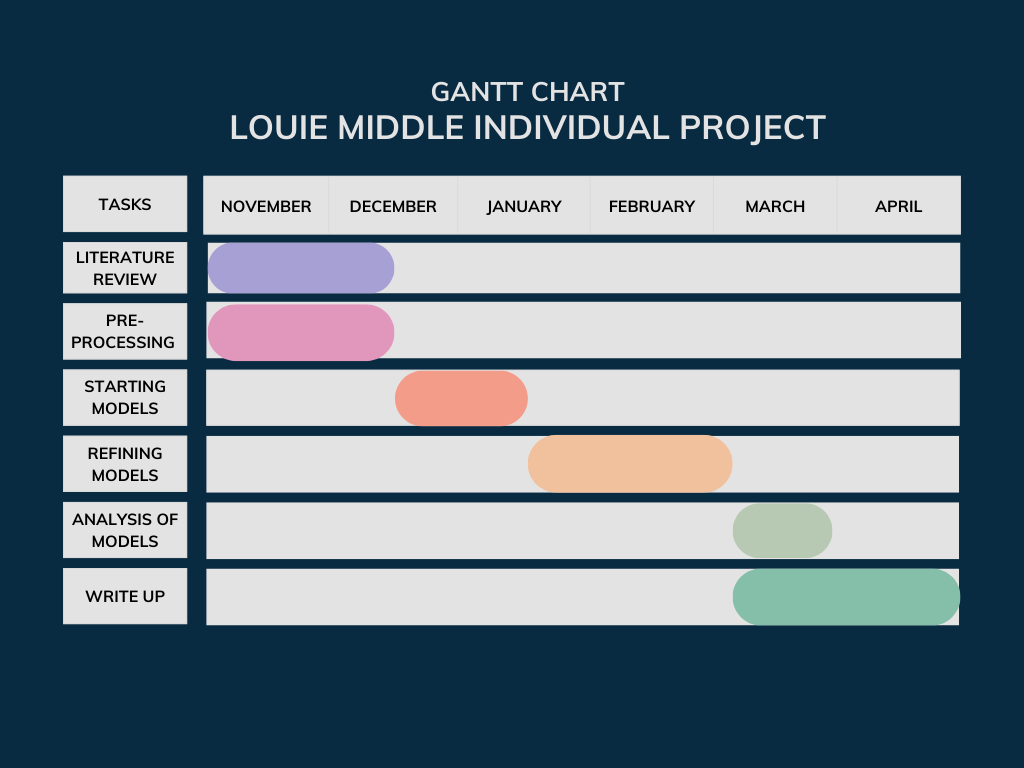
\includegraphics[width=\linewidth]{Gantt Chart.png}
%    \caption{Gantt Chart For Project}
%    \label{fig:gantt_chart}
%\end{figure}
%
%\section{Resources Required}
%
%In order to train any machine learning model an appropriate amount of data for training and testing. 
%Because it is not beneficial to use data that is too old \citep{horvat2020}, at least a recent season's worth of data would be good, saving some data for testing. 
%
%Training machine learning models may also require appropriate computing power depending on the models used and size of the data set. 
%This could potentially be achieved with the University of Bath's Hex GPU cluster.

%%%%%%%%%%%%%%%%%%%%%%%%%%%%%%%%%%%%%%%%%%%%%%%%%%%%%%%%%%%%%%%%%%%%%%%%%%%%%%%%
%%%%%%%%%%%%%%%%%%%%%%%%%%%%%%%%%%%%%%%%%%%%%%%%%%%%%%%%%%%%%%%%%%%%%%%%%%%%%%%%
\chapter{Literature and Technology Survey}

\section{Moneyball}

The release of the book Moneyball \citep{Moneyball2004} and its subsequent film adaptation, was a big driver in the increased use of statistical driven techniques in Baseball player selection and scouting techniques. 
Pioneered by the likes of Bill James and Sabermetrics, Moneyball has entered baseball's lexicon; teams that value Sabermetrics are often said to be playing "Moneyball".  
One of the notable benefits of a Moneyball approach is in reducing player salaries, whilst maintaining high performance. 
Notable recent Moneyball successes include the Tampa Bays, whose entire 2019 roster was around 63\% of the total budget of the \$40 million the Houston Astros were spending on Gerrit Cole's contract. 
It was reported that the Rays spending totalled \$648,000 per victory, compared to the Astros \$1.54 million per win.
Despite this large difference in pay, the Rays still had a successful season and finished second in the American League East \citep{Fox2019}.

Similar successes can be found in other sports, such as association football (or soccer). 
In 2010 Liverpool F.C. were purchased by Boston Red Sox owner John W. Henry. 
During this time with the Red Sox, Henry hired Sabermetrics pioneer Bill James and their Moneyball approach saw the team win the World Series in 2004, 2007, 2013 and 2018. 
Attempting to replicate these results with Liverpool, Henry hired University of Cambridge PhD Ian Graham in 2012 as head of analysis and J\"urgen Klopp as Manager in 2015 \citep{Liverpool2022}. 
Graham influenced the signings of key players, such as Mohammed Salah, Philippe Coutinho and Naby Ke\"ita. 
Graham's data suggested Salah would pair especially well with Roberto Firmino, who creates more expected goals than nearly anyone else in his position \citep{Liverpool2019}. 
Expected goals turned to real goals in the 2017-2018 season, with Salah scoring 32 goals and Firmino scoring 15. 
The combination of Klopp and his intuitive knowledge, paired with the likes of Grahams data-driven knowledge, has led to Liverpool having fantastic recent success winning the 2018-2019 UEFA Champions League and the 2019-2020 English Premier League.

\section{T20 Cricket} \label{sec:T20Cricket}

Whilst there are varying formats of cricket \footnote{Whilst knowledge of cricket is useful to understand this project, it is not necessary to appreciate the project and its applications. Despite this, I present a brief introduction to the game and its laws for those unfamiliar with the sport in chapter \ref{chap:CrickBackground}.}, the focus in this project is the T20 format (20 over cricket) that is played in the IPL.
T20 cricket gives the first team 20 overs to score as many runs as possible, or until they have used all 10 of their wickets.
The teams then swap roles and the opposing team attempt to "chase" the total runs plus one scored by the first team. 
If they manage to do so they win the match, but if all their batters get out before the target total, or use all 20 overs before reaching the target, they lose.

Longer formats of the game such as 40/50 over one day matches and four/five day matches have different tactics compared to T20 cricket.
Due to T20s shorter nature, a bowling team's goal is generally to minimise the runs the batting team can score, in addition to the traditional goal of taking wickets.
Typically, once a batter settles into their innings they attempt to score more boundaries to maximise the runs scored in the short playing period.
Furthermore, some "power hitters" are selected for their specialism in scoring boundaries (see \ref{sec:Boundaries}) at the end of an innings, with no "settling in" period that is afforded to batters in longer formats or at the start of a T20 innings.
Whilst this style of play is more risky as the chances of misplaying increase, it is generally more beneficial to score as many runs as possible in the short time T20 cricket allots.
In general T20 batters protect their wicket less than those in other formats and play a riskier, high run scoring style of play.
\citet{Irvine2017} and the general consensus of the cricket community is that this high boundary scoring carries a greater importance than scoring singles (see \ref{sec:Runs}). 
\citet{Irvine2017} found that the higher the number of singles scored was detrimental to a batting team's chances of success.

Due to the batters desire to score boundaries in T20, bowlers might adopt different strategies to reduce the batters ability to score boundaries. 
This is often done through bowling a wider variety of deliveries and aiming for dot balls (see \ref{sec:Runs}) or singles.
Consequently, this should reduce the runs the batters score and increase the chance of taking a wicket due to the batter needing to play a wider variety of shots to score runs, which increases the chance of them making a mistake.
In general, T20 bowling attacks often assess the ways to reduce the number of boundaries the opposing team can score.
\citet{Irvine2017} found that increased number of dot balls led to a higher chance of winning for the bowling team. 

\subsection{Indian Premier League} \label{sec:IPL}

The Indian Premier League (IPL) is a professional cricket league based on the T20 format.
As reported by \citet{ESPNcricinfo2018}, Star Sports invested \$2.55 billion for exclusive broadcasting rights for the 2018 IPL season. 
This season saw a 29\% increment in the number of viewers, through both digital streaming and television. 
The interest in the IPL is clear.
This increases the desire to use modern machine learning techniques to improve results.

\section{Existing Machine Learning Research on Sport} \label{sec:SportSurvey}

\begin{figure}[H]
    \centering
    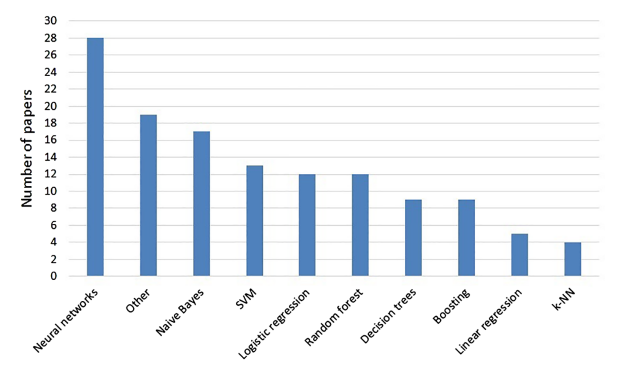
\includegraphics[width=\linewidth]{Horvat&Job_Figure2.png}
    \caption{Total number of papers using a particular ML algorithm group \citep{horvat2020}}
    \label{fig:NoPapers}
\end{figure}

Figure \ref{fig:NoPapers} from \citet{horvat2020}'s literature review of machine learning in sport for score prediction show the methods that are currently used in the field as of May 2020. 
As shown in the figure, neural networks have a large research output.
This is followed by other popular methods such as regression, support vector machines (SVMs), regression, decision trees, and gradient boosting, with k-nearest-neighbours (k-NN) being the least used. 
It is important to note that whilst a larger body of research has been carried out with certain methods, it does not necessarily mean they are the optimal method.

\citet{horvat2020} also showed that including excessive seasons worth of data for training models reduces the quality of results. 
To those with a basic knowledge of cricket and sport this is not surprising given that in just a few years, many factors relating to team composition and tactics can change. 
The most accurate results were achieved by researchers who used data from a single season and a data segmentation evaluation method. 
When using data from a single season, the majority of the data was used for training and a small portion for testing. 
Some researchers used the same data set for training and testing, yielding unrealistically accurate results.

\subsection{Expected Goals and Football}

Expected goals (xG) is a statistical metric used in football to quantify the quality of scoring chances created by a team or player in a match. 
Each shot is assigned a probability of being scored, which is calculated by analysing a range of variables such as shot location, shot angle, distance from goal, type of shot, and more. 
This can be done with traditional statistical methods, or machine learning approaches.
Expected goals provides a more accurate assessment of a team's performance than simply looking at the number of goals scored as it takes into account the quality of the chances made.

Large sports analysis company StatsBomb have referenced in their blog posts that their xG model uses gradient boosting models \citep{statsbomb2022}. 
This can also be seen in that when \citet{Blumberg2020} implemented his own xG model, he made use of XGBoost \citep{Chen2016} and achieved comparable results to StatsBomb.
One of the valuable things about XGBoost and Blumbergs model is that it provides a feature interpretation of what features are most important.

\section{Existing Machine Learning Research on Cricket} \label{sec:CrickSurvey}

\citet{KampakisStylianos2015} used Naïve Bayes, logistic regression, random forests and gradient boosted decision trees to predict the outcome of English County 20 over Cricket Matches from 2009 - 2014. 
The performance of each algorithm was assessed using one year's data as the training data set and the following year's data for testing. 
Each model was tested over these seasons and achieved an accuracy of 62.4\% for Naïve Bayes, 60.1\% for logistic regression, 55.6\% for random forests and 57.2\% for decision trees.

\begin{table}[H] \label{tab:ResearchCrick}
	\centering
	\caption{Research areas in cricket and their percentage of the total research output in cricket \citep{Wickramasinghe2022}}
	\begin{tabular}{| c | c |} 
		\hline
		Research Area & \% of Studies \\ [0.5ex] 
		\hline\hline
		Game Outcome Prediction & 35 \\ 
		\hline
		Player's Performance Classification & 16 \\
		\hline
		Batting Style/Stroke Classification & 9 \\
		\hline
		Other & 9 \\
		\hline
		Umpire's Decision/Gestures & 6 \\
		\hline
		Score Prediction & 5 \\
		\hline
		Cricket Commentary/Media & 4 \\
		\hline
		Pitch Behaviour Predicition & 4 \\
		\hline
		Team Selection/Performance & 3 \\ [1ex] 
		\hline
	\end{tabular}
\end{table}

\citet{Wickramasinghe2022} review of machine learning in cricket from December 2022 classified the current areas of research in cricket. 
He found that over half of studies aim to predict the outcome of a game, or classify different players performances. 
The full table of results can be seen in table \ref{tab:ResearchCrick}. 
From this it is clear to see that there is very little research in predicting batter bowler matchups or the outcome of a single delivery. 
Instead, most of the focus is on predicting game outcomes or overall player performance.

\begin{figure}[H]
    \centering
    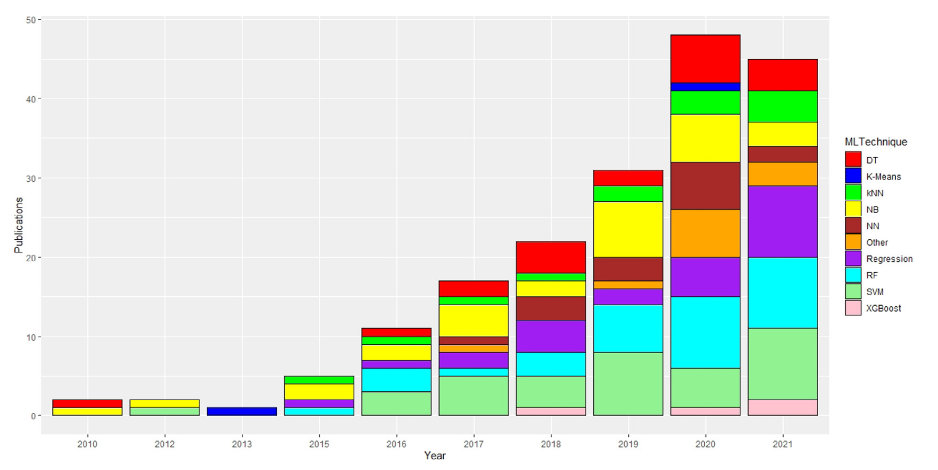
\includegraphics[width=\linewidth]{ML_techniques_cricket.png}
    \caption{Total number of publications for each ML technique each year in cricket research \citep{Wickramasinghe2022}}
    \label{fig:NoPapersCricket}
\end{figure}

\citet{Wickramasinghe2022} also evaluated the frequently used ML techniques in cricket, as shown in figure \ref{fig:NoPapersCricket}. 
There is a noticeable lack of deep learning or reinforcement learning techniques.
Furthermore, better boosting algorithms such as XGBoost have only recently begun to be adopted and Gaussian processes have not been used at all.
There is clearly gaps in currently research methods in sports analytics.

Lastly, a clear uptick in the number of publications can be seen over the years, which is also corroborated in sport as whole in \citet{horvat2020}.
It once again highlights the growing interest in ML in sport.

\subsection{Existing Machine Learning Research on the Indian Premier League}

\citet{Saikia2012} have used Artificial Neural Network models to predict the performance of bowlers based on their performance in the first three seasons of the IPL. 
When the predicted results were validated with the players performances in the fourth season, the model had an accuracy of 71.43\%.

Otherwise, there is generally limited research on the IPL and it is an area ripe for research.

%\subsection{Expected Runs}
%
%In cricket, expected runs (xR) refers to the estimated number of runs a team or a batsman is expected to score based on various factors such as the number of overs left, the current score, and the quality of the opposition. 
%It is calculated using statistical models that take into account various variables such as the batsman's average, strike rate, and the pitch conditions. 
%The concept of expected runs is often used by cricket analysts and commentators to assess a team's performance, identify areas of improvement, and make predictions about the outcome of a match. 
%It is a useful tool in evaluating a player's performance and predicting the final score of a match.
%
%TODO: Talk about CricketSavant, his XGBoost, and then subsequent hiring by CrickVis.

\section{Research With Similar Goals}

The Singlearity-PA model \citep{silver2021baseball} wanted to attempt to solve one of the most fundamental questions in baseball:	 How can we	predict the outcome of a batter	vs. pitcher plate appearance (PA)? 
This is similar to my goal with cricket: To predict the outcome of batter vs bowler.

The Singlearity-PA model \citep{silver2021baseball} was able to accurately predict the results of a batter versus pitcher plate appearance using a neural-network based AI model. 
The details of the model used are vague, however the network was able to take in 87 inputs and then output probabilities for each of the 21 possible outcomes of a plate appearance (PA) in baseball. 
Comparisons can be made between this and cricket. 
A plate appearance can be compared to an over, comprising 6 balls (or more including no balls and wides) between a single bowler and 1 or more batsmen. 
The outcome of the over could be considered to be the runs scored. 

\citet{silver2021baseball} also split their player base up by how many PAs they had for each player. 
The best players had greater than 500 PAs worth of data each, but the vast majority had less than 100. 
SinglearityPA was able to accurately predict the result of match-ups for these players with fewer PAs better than existing solutions. 
Parallels can be drawn between this and cricket, as there are often players who have little data, yet team selectors would want to know who the best player is to match-up against them.

Extending Singlearity-PA with Markov chains improved more complicated strategies, such as optimal player lineups or to decide on pinch hitters and relief pitchers. 
Similarly, in cricket the batting lineup and choice of bowler at different points in a game have a large impact on the score. 
In the example provided, Singlearity-PA's predicted runs scored for an optimal lineup was 6.7\% better than the actual lineup in the 2019 National League All-Star game. 
It is important not to compare baseball and cricket too closely, but the techniques used by Silver and Huffman could potentially work well in Cricket.

%\section{Gaussian Processes in Sport}
%
%TODO: Talk about Gaussian processes in sport

\chapter{Background}

This chapter will firstly introduce some background on Hawk-Eye and current computer vision in sports.
Next, the requisite background for Gaussian processes and gradient boosting, the two key methods used in this project is provided.
Additionaly, the idea of a data association problem is introduced. 

\section{Hawk-Eye and Ball Tracking}

The dataset used in this project contains tracking data from Hawk-Eye systems.
Hawk-Eye Innovations is a sports technology company, that provides many products, including computer version services.
In particular there is a focus on ball and player tracking in sports, including cricket.
In this project the emphasis is placed on the ball tracking.
Hawk-Eye have a number of cameras at IPL grounds, that the video from is then triangulated and combined to create a three-dimensional representation of the ball's trajectory.
It has been adopted as an ajudication tool by many governing bodies in cricket and is generally accepted to be accurate.

Hawk-Eye tracking data is accumulated and stored. 
It can then be used for various data science and machine learning purposes.
Further explanation of the dataset and features used in this project are explained in section \ref{sec:Dataset}.

\section{Gaussian Processes}

\citep{Yi2019} TODO: This has good explanations of stuff

\citep{Griffiths2023} TODO: As does this

This section introduces Gaussian processes and the following section then explains how to extend their application to solve data association problems. 
A background on using Gaussian processes for regression is provided first as a basis before their extension to classification tasks. 
As Gaussian processes are not computationally cheap, sparse approximations are also reviewed in this section.

Gaussian processes are a non-parametric regression model. 
\emph{Non-parametric models} are not based on insights about the concrete structure of the function to be modelled, but instead make assumptions about the function itself, such as its smoothness or differentiability. 
Instead of modeling a distribution of parameter values, a non-parametric model tries to find a distribution $p(f*)$ of probable functions that represents the function $f$ to be estimated \citep{Kaiser2017}.

In addition, Gaussian processes are a supervised learning technique. 
It starts with a training data set $\mathcal{D}$ of $n$ observations, $\mathcal{D} = (\textbf{x}_{i}, y_{i} | i = 1, ..., n)$.
$\textbf{x}$ denotes an input vector (covariates) of dimension $D$ and $y$ denotes an output or target. 
The column vector inputs for all $n$ cases are aggregated in the $D x n$ design matrix $X$ and the targets collected in the vector $\textbf{y}$, such that $\mathcal{D} = (X, \textbf{y})$ \citep{RasmussenWilliams2006}.

\subsection{Gaussian Processes for Regression}

%\subsubsection{Weight Space View}

%TODO: This section might not be necessary, but might be good to show understanding....

%One can think of a Gaussian process as defining a distribution over functions and inference taking place directly in the space of functions. 
%Although this view is appealing, it is difficult to grasp on first attempt, and so we will start with reviewing the \emph{weight-space view}.
%
%First, lets review the standard linear regression model with Gaussian noise

%\begin{equation}
%    \centering
%    {f(\textbf{x}) = \textbf{x}^T\textbf{w}, \quad y = f(\textbf{x}) + \epsilon}
%\end{equation}

%where $\textbf{x}$ is the input vector, $\textbf{w}$ is a vector of weights of the linear model, $f$ is the function value, and $y$ is the observed target value.
%It is often assumed that the observed values differ from the function values by some noise, which we will treat as an independent, identically distributed Gaussian distribution, with zero mean and variance $\sigma^2_{n}$.

%\begin{equation}
%    \centering
%    \epsilon \sim \mathcal{N}(0, \sigma^2_{n})
%\end{equation}

%This noise assumption together with the model gives rise to the likelihood, the probability density of the observations given the parameters, which is factored over cases in the training set to give

%\begin{equation}
%    \centering
%    p(\textbf{y} | X, \textbf{w}) = \prod_{i=1}^n = p(y_{i} | \textbf{x}_{i}, \textbf{w}) =  \prod_{i=1}^n \frac{1}{\sqrt{2\pi}\sigma_{n}} exp(-\frac{(y_{i} - \textbf{x}_{i}^T \textbf{w})^2}{2 \sigma_{n}^2})
%    TODO: Can do the rest later
%\end{equation}

%We put a zero mean Gaussian prior with covariance matrix $\Sigma_{p}$ on the weights 
%
%\begin{equation}
%    \centering
%    \textbf{w} \sim \mathcal{N}(0, \Sigma_{p})
%\end{equation}
%
%Inference is based on the posterior distribution over the weights computed by Baye's rule, given by
%
%\begin{equation}
%	\centering
%	P(\textbf{w} | \textbf{y}, X)  = \frac{p(\textbf{y} | X, \textbf{w})p(\textbf{w})}{p(\textbf{y} | X)}
%\end{equation}
%
%Note that prior $p(\textbf{w})$ neglects the conditioning on $X$, as it is independent of the inputs. The normalising constant $p(\textbf{y} | X)$, also know as the marginal likelihood is independent of the weights and is given by
%
%\begin{equation}
%	\centering
%	P(\textbf{y} | X)  = \int p(\textbf{y} | X, \textbf{w})p(\textbf{w}) d\textbf{w}
%\end{equation}
%
%Since the number of obervations is finite and the function $f$ lives in an infinite dimensional function space, the estimation of $f$ is uncertain and based on prior assumptions about its structure.
%
%TODO: Finish this later when you can ask Adam about it....
%
%To make predictions we average over all possible parameter values, weighted by their posterior probability.
%Thus the predictive distribution for $f_{*} \triangleq f(\textbf{x}_{*})$ at $\textbf{x}_{*}$ is given by averaging the output of all possible linear models w.r.t the Gaussian posterior
%
%\begin{equation}
%	\begin{aligned}
%		\centering 
%		p(f_{*} | \textbf{x}_{*}, X, \textbf{y}) &= \int p(f_{*} | \textbf{x}_{*}, \textbf{w})p(\textbf{w} | X, \textbf{y}) d\textbf{w}\\
%		&= \mathcal{N}(\frac{1}{\sigma_{n}^2} \textbf{x}_{*}^T A^{-1} X \textbf{y}, \enskip \textbf{x}_{*}^T A^{-1} \textbf{x}_{*}).
%	\end{aligned}
%\end{equation}
%
%The predictive distribution is again Gaussian.

\subsubsection{Function-Space View}

\begin{definition}[Gaussian Process]
A Gaussian process is a collection of random variables, any finite number of which have a joint Gaussian distribution. 
\end{definition}

Gaussian processes are a generalisation of the Gaussian distribution to function spaces. 
A multivariate Gaussian $\textbf{x} \sim \mathcal{N} (\boldsymbol{\mu}, \boldsymbol{\Sigma})$ describes a distribution over the finite elements in the vector $\textbf{x}$. 
Every element of $\textbf{x}$ is normally distributed. 
For two points in $\textbf{x}$, $x_{i}$ and $x_{j}$, their covariance is given by $cov[x_{i}, x_{j}] = \Sigma_{ij}$.

A Gaussian process is completely specified by its mean function, $m(\textbf{x})$, and its co-variance function $k(\textbf{x}, \textbf{x}')$.
Usually, the mean function is assumed to be constant zero, but this need not be the case.
A mean function and covariance function can be defined for a real process $f(x)$ as 

\begin{equation}
	\begin{aligned}
		\centering
		m(\textbf{x}) &= \mathbb{E}[f(\textbf{x})],\\
		k(\textbf{x}, \textbf{x}') &= \mathbb{E}[(f(\textbf{x}) - m(\textbf{x}))(f(\textbf{x}') - m(\textbf{x}'))],
	\end{aligned}
\end{equation}

where we will write the Gaussian process as 

\begin{equation}
	\centering
	f(\textbf{x}) \sim GP(m(\textbf{x}), k(\textbf{x}, \textbf{x}')).
\end{equation}

The covariance function, or kernel, specifies the covariance between pairs of random variables. It is the covariance functions which encode the assumptions about the underlying function (see section \ref{sec:Kernels}).

\subsection{Kernels} \label{sec:Kernels}

Kernels are crucial in encoding the assumptions about the function a Gaussian process should estimate. 
It is a measure of similarity of different points in the observed data and of new points to be predicted. 
For example, a natural assumption is that the closer two points lie, the more similar their function values should be. 
Furthermore, when prediciting test points, training points close to it are probably more informative than those further away. 
However, it should be noted this need not be the case. 
For example, consider a sinusoidal wave where two points which are multiple wavelengths apart should have similar function values \citep{Kaiser2017}.
A kernel that only depends on the distance between two points is called \emph{stationary}.
Conversely, kernels that do depend on two points' positions in the input space are called \emph{non-stationary}.

A common kernel and one used throughout this project is the squared exponential (SE) covariance function (also known as the radial basis function, RBF). 
For a finite dimensional input space $\mathbb{R}^d$, the SE kernel is defined by

\begin{equation}
	\centering
	cov(f(\textbf{x}), f(\textbf{x}')) = k(\textbf{x}, \textbf{x}') = \sigma_{f}^2 exp(-\frac{1}{2} (\textbf{x} - \textbf{x}')^T \Lambda^{-1} (\textbf{x} - \textbf{x}')).
	\label{eq:SquaredExponentialKernel}
\end{equation}

Kernels have characteristic length scales which informally can be thought of as roughly the distance you have to move in input space before the function value will change significantly. 
$\Lambda^{-1}  = diag(l_{1}^2, ... , l_{d}^2)$ is a diagonal matrix of the squared length scales $l_{i} \in \mathbb{R}_{>0}$ in each axis.
The variable $\sigma_{f}^2 \in \mathbb{R}_{>0}$ is the signal variance.
The signal variance specifies the average distance of function values from the mean value.
The vector of all hyperparameters in a model is called $\boldsymbol{\theta}$.
Choices of such free hyperparameters will be discussed more in chapter \ref{chap:Method} including their optimisation. 

\begin{figure}[H]
   	 \begin{minipage}[t]{0.3\textwidth}
	 	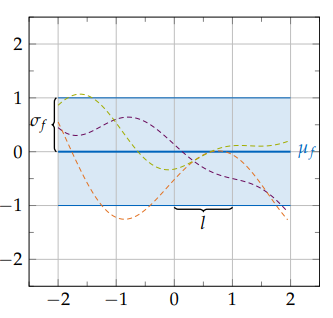
\includegraphics[width=\linewidth]{RBF_sigma_1_lengthscale_1.png}
	    	\caption{SE kernel with $\sigma=1$ and $l=1$ \citep{Kaiser2017}}
	    	\label{fig:SEKernSig1Length1}
	\end{minipage}
	\hfill
	\begin{minipage}[t]{0.3\textwidth}
	 	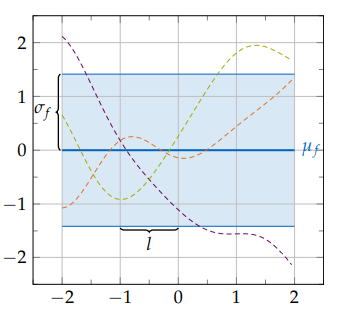
\includegraphics[width=\linewidth]{RBF_sigma_root2_lengthscale_1.png}
	    	\caption{SE kernel with $\sigma=\sqrt{2}$ and $l=1$ \citep{Kaiser2017}}
	    	\label{fig:SEKernSigRoot2Length1}
	\end{minipage}
	\hfill
	\begin{minipage}[t]{0.3\textwidth}
	 	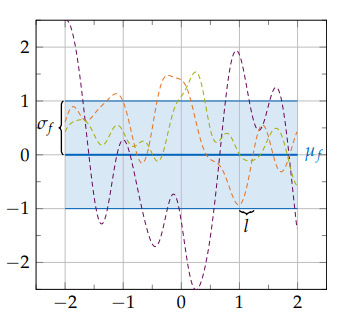
\includegraphics[width=\linewidth]{RBF_sigma_1_lengthscale_025.png}
	    	\caption{SE kernel with $\sigma=1$ and $l=0.25$ \citep{Kaiser2017}}
	    	\label{fig:SEKernSig1Length0.25}
	\end{minipage}
\end{figure}

Figure \ref{fig:SEKernSig1Length1}, figure \ref{fig:SEKernSigRoot2Length1} and figure \ref{fig:SEKernSig1Length0.25} compare sample functions drawn from Gaussian processes with SE kernels with different hyperparameters. 
Since the mean function $m(x)$ is assumed to be constant zero, the kernel specifies the prior assumptions about the function.
The SE kernel describes arbritrary smooth functions. The hyperparameters $l$ and $\sigma$ of the kernel describe the dynamic range in the $x$ and $y$ directions respectively.
As can be seen in figure \ref{fig:SEKernSig1Length0.25}, reducing the length scale increases the curvature of drawn sample functions from the kernel.
Increasing the signal variance as shown in figure \ref{fig:SEKernSigRoot2Length1}, increases the range of values the sample function will take.

\subsection{Predictions and Posterior}

In order to use Gaussian processes for regression, it is necessary to combine observations with a Gaussian process prior $f \sim GP(0, K)$. 
The distribution is obtained by integrating over all possible latent function values $f$ and therefore taking all possible functions into account. This is called the \emph{marginilisation of $f$}. 

The joint distribution of the training outputs, $\textbf{y}$, and the test outputs $\textbf{f}_{*}$ according to the prior is 

\begin{equation}
	\centering
	\begin{bmatrix}
		\textbf{y} \\
		\textbf{f}_{*}
	\end{bmatrix}
	\sim \mathcal{N} \left( 0,
	\begin{bmatrix}
		K(X, X) + \sigma_{n}^2I & K(X, X_{*}) \\
		K(X_{*},  X) & K(X_{*},  X_{*})
	\end{bmatrix} \right) .
	\label{eq:JointPriorDist}
\end{equation}

If there are $n$ training points and $n_{*}$ test points then $K(X, X_{*})$ denotes the $n x n_{*}$ matrix of covariances evaluated at all pairs of training and test points. 
This is the same for $K(X, X)$, $K(X_{*},  X)$ and $K(X_{*},  X_{*})$.

This results in the key predicitve equations for Gaussian process regression

\begin{equation}
	\textbf{f}_{*} | X, \textbf{y}, X_{*} \sim \mathcal{N}(\overline{\textbf{f}}_{*}, cov(\textbf{f}_{*}))
\end{equation}
\begin{equation}
	\overline{\textbf{f}}_{*} \triangleq \mathbb{E}[\textbf{f}_{*} | X, \textbf{y}, X_{*}] = K(X, X_{*})[K(X, X) +  \sigma_{n}^2I]^-1 \textbf{y}
	\label{eq:MeanFunc}
\end{equation}
\begin{equation}
	cov(\textbf{f}_{*}) = K(X_{*}, X_{*}) - K(X_{*}, X)[K(X, X) +  \sigma_{n}^2I]^-1 K(X, X_{*}).
	\label{eq:CovarianceFunc}
\end{equation}

Eq. \ref{eq:MeanFunc} and eq. \ref{eq:CovarianceFunc} represent the mean function and the covariance function of the Gaussian posterior process respectively. 

Accordingly a compact form of $K(X, X)$ and $K(X_{*}, X_{*})$ etc. will be introduced where $K = K(X, X)$ and $K_{*} = K(X, X_{*})$.

\subsubsection{Marginal Likelihood}

The marginal likelihood is the marginalisation over the function values $\textbf{f}$. 
Observing that $\textbf{y} \sim \mathcal{N} (0, K + \sigma_{n}^2I)$ yields the log marginal likelihood

\begin{equation}
	\label{eq:LogMargLik}
	\centering
	\log p(\textbf{y} | X) = -\frac{1}{2}\textbf{y}^T(K +  \sigma_{n}^2I)^-1\textbf{y} - -\frac{1}{2}log|K +  \sigma_{n}^2I| - \frac{n}{2}log2\pi.
\end{equation}

With this, we can create an algorithm for Gaussian process regression, which is given in alg. \ref{alg:GPR}. The matrix inversion required by eq. \ref{eq:MeanFunc} and \ref{eq:CovarianceFunc} uses Cholesky factorisation, explained in section \ref{sec:CholFac}. 

\begin{algorithm}
	\caption{Algorithm for Gaussian process regression \citep{RasmussenWilliams2006}}
	\label{alg:GPR}
	\begin{algorithmic}[1]
		\Require $X$ (inputs), \textbf{y} (targets), $k$ (covariance function), $\sigma_{n}^2$ (noise level), $X_{*}$ (test input)	
		\State $L \gets cholesky(K +\sigma_{n}^2I)$
		\State $\boldsymbol{\alpha} \gets L^T \setminus (L \setminus \textbf{y})$ \Comment{eq. \ref{eq:MeanFunc}}
		\State $\overline{f}_{*} \gets \textbf{k}_{*}^T \boldsymbol{\alpha}$ \Comment{eq. \ref{eq:MeanFunc}}
		\State $\textbf{v} \gets L \setminus \textbf{k}_{*}$ \Comment{eq. \ref{eq:CovarianceFunc}}
		\State $\mathbb{V}[f_{*}] \gets k(X_{*}, X_{*}) - \textbf{v}^T\textbf{v}$ \Comment{eq. \ref{eq:CovarianceFunc}}
		\State $\log p(\textbf{y} | X) \gets -\frac{1}{2} \textbf{y}^T \boldsymbol{\alpha} - \Sigma_{i} \log L_{ii} - \frac{n}{2} \log2\pi$ \Comment{eq. \ref{eq:LogMargLik}}
		\State \textbf{return}: $\overline{f}_{*}$ (mean), $\mathbb{V}[f_{*}]$ (variance), $\log p(\textbf{y} | X)$ (log marginal likelihood)
	\end{algorithmic}
\end{algorithm}

\subsubsection{Loss Functions}

For practical applications, there must be a decision on how to act - a point prediction is necessary. 
To achieve this, we need a loss function $\mathcal{L}(y_{true}, y_{guess})$ which specifies the loss incurred by guessing the value $y_{guess}$ when the true value is $y_{true}$. 
The goal is to then make the point predicition $y_{guess}$ that incurs the smallest loss.
This can be done by minimising the expected loss or risk by averaging w.r.t. our model what the truth might be.
Thus the best guess is 

\begin{equation}
	\centering
	y_{optimal} | \textbf{x}_{*} = \underset{y_{guess}}{\textrm{argmin}} \, \overset{\sim}{R_{\mathcal{L}}}(y_{guess} | \textbf{x}_{*})
\end{equation}

where $\overset{\sim}{R_{\mathcal{L}}}$ represents the risk and $\overset{\sim}{R_{\mathcal{L}}}(y_{guess} | \textbf{x}_{*}) = \int \mathcal{L}(y_{*}, y_{guess}) p(y_{*} | x_{*}, \mathcal{D}) dy_{*}$ \citep{RasmussenWilliams2006}.

\subsubsection{Choosing Hyperparameters}

Up until now, the hyperparameters $\boldsymbol{\theta}$ have been assumed constant.
If this were the case, GPs would have no training stage. 
However, knowing the correct hyperparameters is not clear a priori, and so a method of determing the hyperparameters must be used.

The correct way to model uncertainty about the hyperparameters is to give them a prior probability $p(\boldsymbol{\theta})$.
The prior chosen should be broad to reflect the vagueness of the parameters before training.
To derive the dependent distributions marginalise the prior to get

\begin{equation}
	\begin{aligned}
		\centering
		p(f) &= \int p(f | \theta) p(\theta) d\theta \\
		p(y | X) &= \int p(y | X, \theta) p(\theta) d\theta.
	\end{aligned}
\end{equation}

A new distribution can be obtained by combining the prior with the likelihood of the training data observed using Baye's theorem:

\begin{equation}
	\label{eq:ChooseHyper}
	\begin{aligned}
		\centering
		p(\boldsymbol{\theta} | X, y) &= \frac{p(y | X, \theta) p(\theta)}{p(y | X)} \\
		&= \frac{p(y | X, \theta) p(\theta)}{\int p(y | X, \theta) p(\theta) d\theta} 
	\end{aligned}
\end{equation}

The integration required in the denominator of eq. \ref{eq:ChooseHyper} is very hard in practise as $y$ is a complicated function of $\boldsymbol{\theta}$. 
Instead, $p(\boldsymbol{\theta} | X, y)$ is maximised to provide an estimate and does not require the calculation of the integral in the denonimator because it is a constant.
The solution of the numerator $p(y | X, \theta)$ you might recognise as the log marginal likelihood in eq. \ref{eq:LogMargLik}. 
For practical reasons minimising the negative of the log marginal likelihood is easier than maximising it directly.
Therefore, the estimation of hyperparameters is the solution of the following optimisation problem:

\begin{equation}
	\centering
	\boldsymbol{\theta}^* \in \underset{\boldsymbol{\theta}}{\textrm{argmin}} \, -p(y | X, \theta).
\end{equation}

\subsection{Gaussian Processes for Classification}

A Gaussian process is a generalisation of the Gaussian probability distribution. 
Both classification and regression can be seen as function approximation problems. 
Unfortunately, the solution of classification problems using Gaussian processes is tougher than regression problems. 
For regression problems, the likelihood is often assumed to be Gaussian. 
A Gaussian process prior combined with a Gaussian likelihood gives a posterior Gaussian process over functions, where everything remains analytically tractable. 
For classification models, the Gaussian likelihood is inappropriate; a different likelihood such as a Bernoulli or multi-class likelihood must be used.
When the likelihood is non-Gaussian, the bayes rule results in an intractable posterior $p(f|y)$ \citep{Yi2020}.
However, a variational approach can approximate the true posterior distribution.

%In such cases the latent function $f$ plays the role of a nuisance function. 
%This is that values of $f$ are not observed directly and there is no interest in the values of f, but rather in $\pi$ where $\pi (\textbf{x})$ is TODO.
%The purpose of $f$ is solely to allow convenient formulation of the model and the goal is to integrate out $f$.
%TODO: Fill out this paragraph.

\subsection{Variational Gaussian Processes}

Variational Gaussian processes (VGP) models use a variational approximation to the true posterior distribution over functions.
The variational approach in VGP models involves approximating the true posterior distribution with a simpler, tractable distribution. 
This distribution is the variational distribution and $q(f)$ is used to denote its probability density function.
This forces some key assumptions, namely that there exists some concrete variational distribution that is similar to the true posterior distribution. 
Next is that we can find the parameters for this approximate distribution in some way \citep{Yi2020}.

Ultimately, the parameters of this approximate distribution are optimised to minimise the Kullback-Leibler (KL) divergence (see section \ref{sec:KLDiv} for an overview) between the approximate and true posterior distributions, where the KL divergence signifies the closeness between the two distributions.
Gradient descent maximises the expression for the evidence lower bound (ELBO) to find concrete model parameter values.

\subsection{Sparse Variational Gaussian Processes}

A major drawback of Gaussian processes is their $O(N^3)$ complexity when computing $[K + \sigma_{n}^2I]^{-1}$ from alg. \ref{alg:GPR}, but it can be done as a preprocessing step since it is independent of the test points. 
After this, each single test point costs $O(N)$. 
To predict its variance it is still necessary to perform matrix multiplication which costs $O(N^2)$.
Consequently, as the size of the dataset grows the more infeasible it is to evaluate a GP.

An approach to reduce this complexity is \emph{Sparse Variational Gaussian Processes} (SVGP) \citep{Hensman2014}.
Spare approximations of GPs are a method of approximating a GP using a $M < N$ set of \emph{inducing points} $\textbf{Z}$ and \emph{inducing variables} $\textbf{u}$ that can represent the entire dataset, rather than $X$ itself. 
This approach suits datasets with high levels of redundancy, but also introduces the problem of choosing the subset.

Using inducing points, we arrive at the Nystr{\"o}m approximation

\begin{equation}
	K_{NN} \approx K_{NM} K_{MM}^-1 K_{MN},
\end{equation}

where $K_{NM} = K(\textbf{X}, \textbf{Z})$ and $K_{MM} = K(\textbf{Z}, \textbf{Z})$.
The SVGP complexity now costs $O(NM^2)$ instead of $O(N^3)$ \citep{Lui2020}.

When the inducing points are the real data points, such that $\textbf{Z} = \textbf{X}$ then $K_{NM} = K_{MM} = K_{NN}$ and the bound on the marginal likelihood becomes tight. 
Therefore, the approximate marginal likelihood equals the real marginal likelihood \citep{Hensman2014}.

The SVGP approach has been shown to provide accurate predictions with significantly reduced computational cost. 
Additionally, it also allows for more efficient training of GP models using stochastic gradient descent.
Lastly, it allows for variational inference, accepting non-Gaussian likelihoods.
For these reasons, it is a popular choice in Gaussian process models \citep{SVGPYi2020}.

\subsubsection{Choosing the Inducing Points}

When choosing your inducing points you want to use a method that will select $M$ inducing points, that can represent the $N$ real points.
This can be done in many ways; an obvious example is to select inducing points linearly across the input range. 
However if your input data is not linearly spaced, then this can misrepresent your data.
A better method used in this project and used in \citet{Hensman2014} is k-means clustering, which can appropriately find all major regions of the input space so long as there are enough inducing points.

TODO: Maybe visualise this?

\section{Data Association}

\begin{figure}[H]
    \centering
    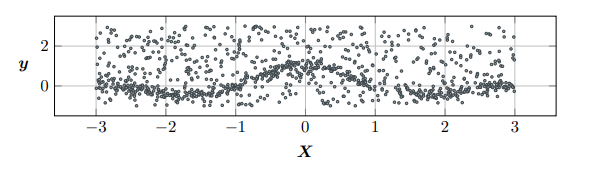
\includegraphics[width=\linewidth]{data_association_problem.png}
    \caption{A data association problem consisting of two generating processes, one of which is a signal to recover and one is an uncorrelated noise process \citep{Kaiser2018}}
    \label{fig:DataAssocProblem}
\end{figure}

A \emph{data association problem} is one where we consider the data to have been generated by a mixture of processes and we are interested in factorising the data into these components. 
For example, as described by \citet{Kaiser2018}, figure \ref{fig:DataAssocProblem} could represent faulty sensor data, where sensor readings are disturbed by uncorrelated and asymettric noise. 
Standard machine learning approaches can pollute any models, where the model starts to explain the noise instead of the underlying signal. 

\subsection{Data Association and Cricket}

The cricket dataset could be deemed a data association problem, as perhaps we can say that each outcome (runs scored) of a cricket delivery is generated by a different process. 
Each of these processes are noisy, as cricket has stochastic outcomes. 

Furthermore, the relationship between a cricket delivery's features and its outcome is not a simple relationship. 
For example, the bowlers length of pitch in IPL cricket (the "pitchY" feature in the dataset) is not a simple case of fuller or shorter is better.
A good short ball from a quick bowler is one that pitches and then reaches the batsmen at shoulder or above height. 
A good yorker is a ball pitching right at the batsmens feets. 
A "good length" delivery is one that pitches and then will pass the stumps at around the top of off stump.
Yet, pitch lengths in between these values are generally considered bad. 
Similar examples can be made with the width of a ball, its swing, its spin, and many other features.

%Equally, a "good" or "bad" ball is subjective depending on the match state and what the bowling team is trying to achieve. 
%Typically in an IPL match the goal of the bowling team is to reduce the oppositions runs scored. 
%The best balls for this requirement are not the same as the best balls to take a wicket. 
%Equally there is an idea in cricket of "setting a batsmen up". 
%This idea refers to having the previous deliveries set the batsmen up to get out on the next ball. 
%For example, a short ball to throw the batsmen off, followed by a yorker right at the stumps. 
%This highlights that there is some relationship between previous deliveries on any future deliveries.

It is clear that the game of cricket has many nuances and challenges for modelling with machine learning techniques. 
Data association techniques however, provide a framework to attempt to seperate some of the differences in how runs are scored in cricket, and model the overlap in the varying outcomes.

\section{XGBoost}

XGBoost is a scalable machine learning gradient boosting library.  
It is an extremely popular, versatile and state-of-the-art gradient boosting technique.
For example, among the 29 challenge winning solutions published at Kaggle’s blog during 2015, 17 of the solutions used XGBoost.
Among these solutions, eight solely used XGBoost to train the model, while most others combined XGBoost with neural nets in ensembles.
The solutions demonstrated that XGBoost gives state-of-the-art results on a wide range of problems, including: store sales prediction; high energy physics event classification; web text classification; customer behavior prediction; motion detection; ad click through rate prediction; malware classification; product categorisation; hazard risk prediction; massive online course dropout rate prediction \citep{Chen2016}.

The versatility and performance of XGBoost make it a popular choice of boosting algorithm, yet it hasn't been widely adopted in cricket research (see section \ref{sec:CrickSurvey}).
For this reason, I wanted to experiment with XGBoost in this project and use it as a baseline performance compared to solutions with GPs.

%%%%%%%%%%%%%%%%%%%%%%%%%%%%%%%%%%%%%%%%%%%%%%%%%%%%%%%%%%%%%%%%%%%%%%%%%%%%%%%%
%%%%%%%%%%%%%%%%%%%%%%%%%%%%%%%%%%%%%%%%%%%%%%%%%%%%%%%%%%%%%%%%%%%%%%%%%%%%%%%%
\chapter{Method} \label{chap:Method}

\section{Objectives}

Following on from the appropriate literature review and background, the primary objectives of this project can be listed as follows:

\begin{enumerate}
  \item From \ref{sec:T20Cricket} it is clear that it is key for bowling attacks to reduce the number of boundaries scored and increase the number of dot balls.
Therefore, a key objective of this project is to accurately predict which delivery would be most optimal to stop a boundary and cause a dot ball or a single.
  \item From sections \ref{sec:SportSurvey} and \ref{sec:CrickSurvey}, it is clear that there is a lack of current research in delivery outcome prediction and use of a wider breadth of ML techniques. 
Another objective of this project, is to attempt to explore new prediciton types in cricket, as well as use under-utilised  ML techniques, notably:
  \begin{enumerate}
	\item Mixtures of Gaussian processes
	\item XGBoost
  \end{enumerate}
\end{enumerate}

\section{Dataset} \label{sec:Dataset}

The dataset used is provided by Hawk-Eye innovations.
At Hawk-Eye's request, the full data-set will not be uploaded due to its commercial sensitivity.
Furthermore, the dataset contains identifying information such as batter names, bowler names, match IDs and so on.
For the purposes of this project and executability of the code submitted, a small subset of the data has been uploaded that I have called the "John Doe dataset". 
This is all the data for one batter, who will be called John Doe from here, that has had any identifying information removed.

The John Doe dataset is a CSV where each row is a different cricket delivery. 
The data includes features such as the bowling style, ball speed, the runs scored (including how many were from the batter or extras), where the ball pitches, where the ball passed the stumps and more.     
The purpose is to use John Doe to explore what the best and worst deliveries are for this person.

\subsection{Features of the dataset}

\subsubsection{Ball Trajectory Features}

\begin{figure}
    \centering
    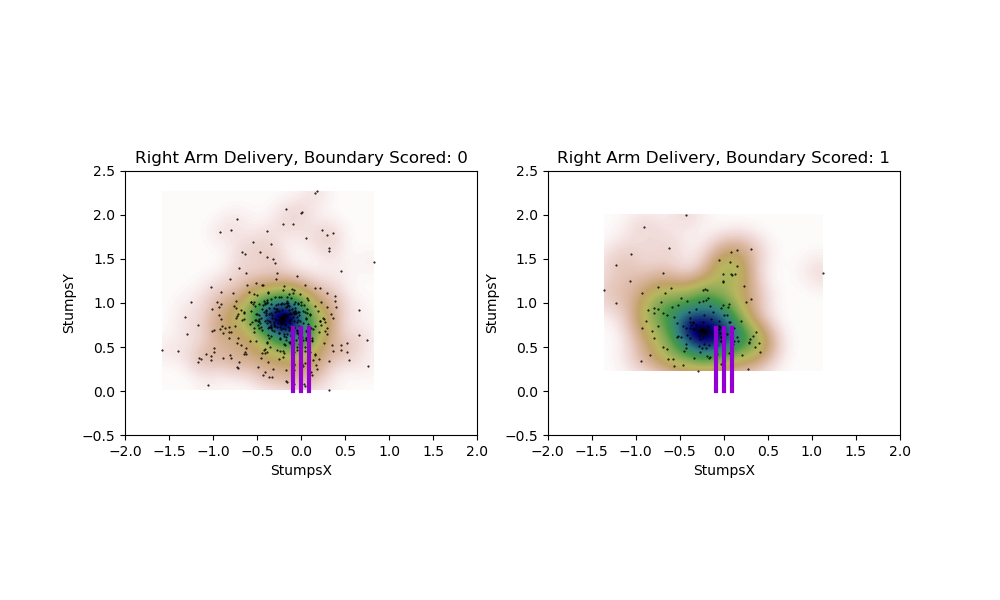
\includegraphics[width=\linewidth]{post_wicket_right_arm.png}
    \caption{The "StumpsX" and "StumpsY" features of the dataset. This is all the right arm seam deliveries faced by John Doe. The left is deliveries that went for 0/1 runs and the right is deliveries that went for 4/6 runs. The purple lines are the stumps if you are looking at the stumps face on.}
    \label{fig:StumpsXY}
\end{figure}

\begin{figure}
    \centering
    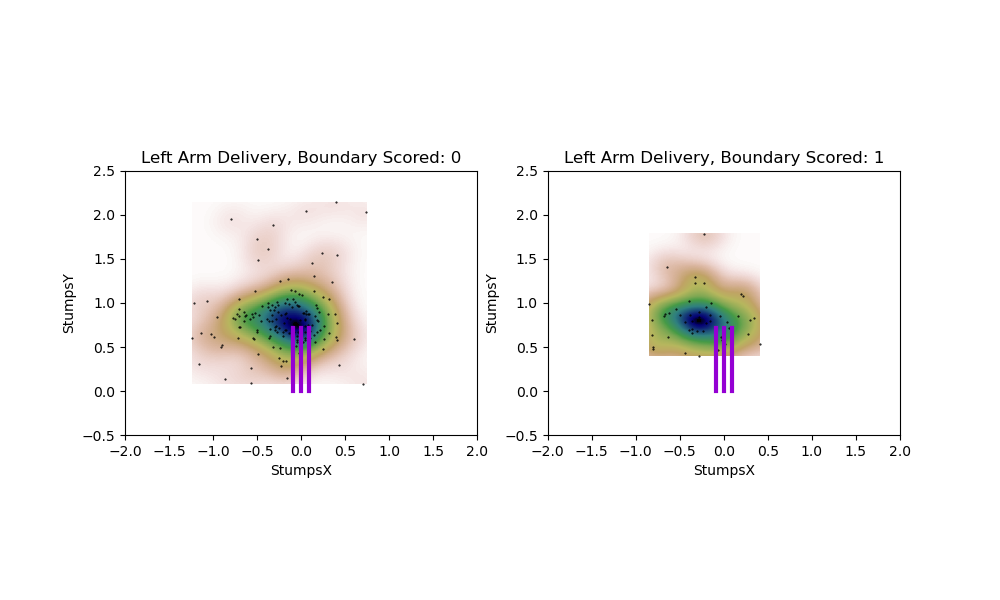
\includegraphics[width=\linewidth]{post_wicket_left_arm.png}
    \caption{The "StumpsX" and "StumpsY" features of the dataset. This is all the left arm seam deliveries faced by John Doe. The left is deliveries that went for 0/1 runs and the right is deliveries that went for 4/6 runs. The purple lines are the stumps if you are looking at the stumps face on.}
    \label{fig:StumpsXY}
\end{figure}

\begin{figure}
    \centering
    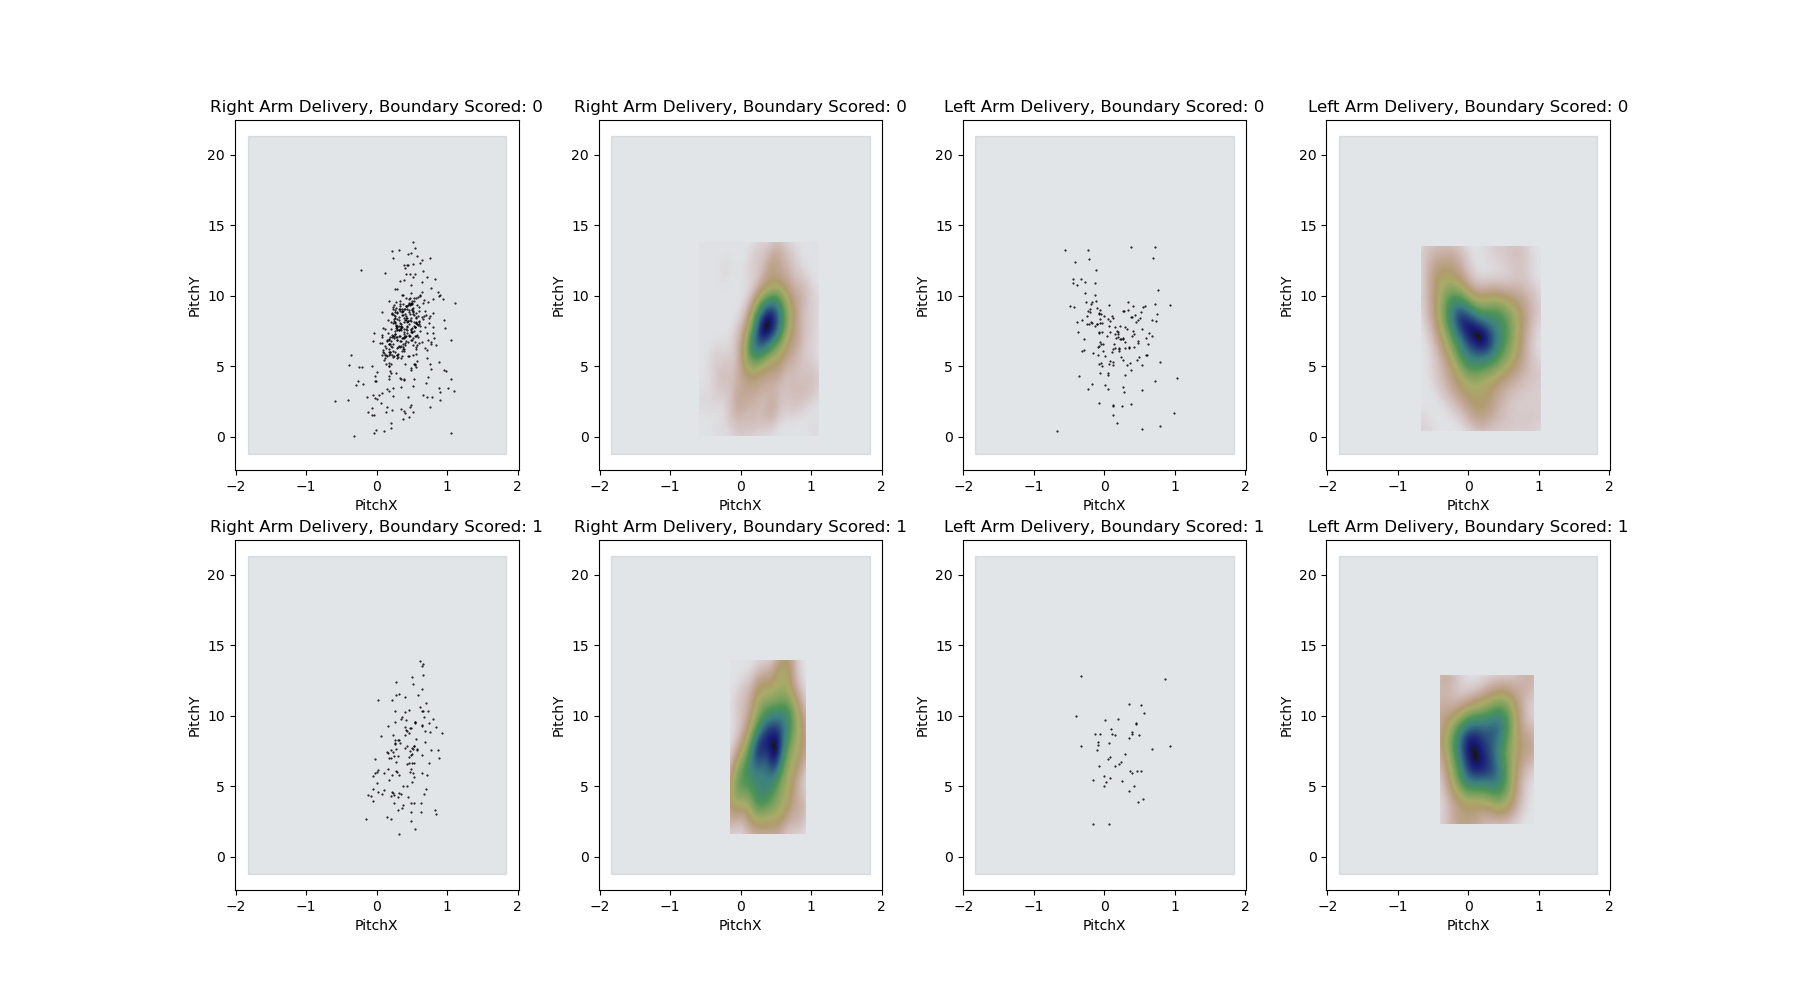
\includegraphics[width=\linewidth]{pitch_bounce.png}
    \caption{The "PitchX" and "PitchY" features of the dataset. This is all the right arm seam deliveries faced by John Doe. The view is birds-eye (from above the stumps). The grey area is the pitch, with the x-axis stretched as to make each delivery clearer.}
    \label{fig:PitchXY}
\end{figure}

\begin{figure}
    \centering
    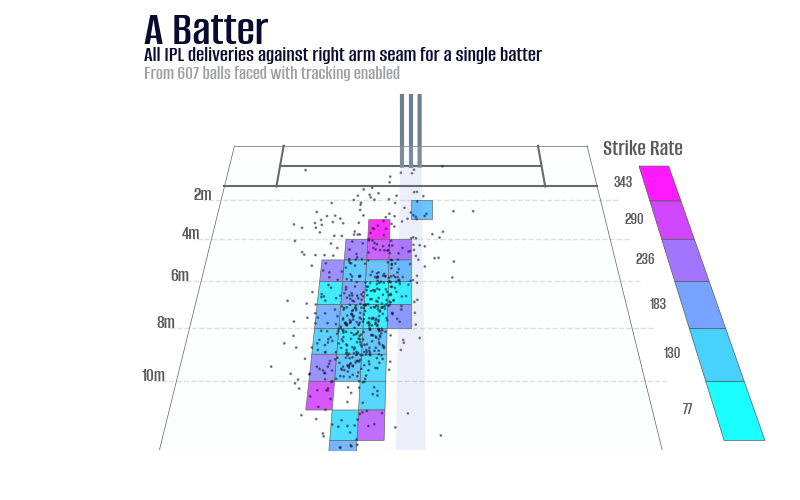
\includegraphics[width=\linewidth]{right_arm_seam_pitch_strike_rate.png}
    \caption{The pitches of right arm seam deliveries for John Doe. For exemplary purposes, the areas on the pitch have been bucketed. Each bucket has an associated strike rate, shown by the scale on the right.}
    \label{fig:PitchXYStrikeRate}
\end{figure}

Figures \ref{fig:StumpsXY} and \ref{fig:PitchXY} visualise the "stumpsX", "stumpsY", "pitchX" and "pitchY" features of the dataset. 
"StumpsX" and "stumpsY" represent where the ball passed the stumps in 2D space.
"PitchX" and "pitchY" represent where the ball bounced on the pitch from a top-down view.
Figure \ref{fig:PitchXYStrikeRate} shows the strike rate \footnote{Strike rate is a common metric in T20 cricket to evaluate a batter's performance. The batters strike rate is their runs scored divided by the balls faced times 100. A high strike rate is good for a batter. Note there is a metric for bowlers also called strike rate that this is not to be confused with.} for the different areas of the pitch. 
It highlights that too short, too wide, or too full deliveries have a higher strike rate than the areas at a classically good pitch length and width.
Whilst it shows that there is potential signs of a good or bad pitch location, one noticeable thing in figures \ref{fig:StumpsXY} and \ref{fig:PitchXY} is how much the data overlaps for different outcomes i.e. locations of no boundary scored are also locations of a boundary being scored.

\subsubsection{Delivery Outcome Features}

To know if a ball was delivered right arm or left arm a "rightArmedBowl" column could take either true or false values.
The following column contained the "bowlingStyle", which included various values such as "FAST\_SEAM", "MEDIUM\_SEAM",  "OFF\_SPIN" and more.
Features for the runs scored also existed, that included "runs", "batterRuns" and "bowlerRuns". 
"BatterRuns" represent runs scored off the batsmen, such as running between the wickets or scoring a boundary.
"BowlerRuns" represent runs scored off the bowler. 
This includes any "batterRuns", but also any additional wides and no balls.
Therefore the column "runs" was a summation of the "batterRuns" and "bowlerRuns", plus any additional cases where the runs will not be attributed to either the batter or bowler, but simply to their respecting teams (for example bys and leg-bys).
The type of extra is indicated in the "extras" column, for example "Wd" (wide) or "Nb" (no ball).

\subsection{Pre-processing}

The first step of the pre-processing was to load all the data into a pandas dataframe and then filter it for one batter.
After that all columns with identifying information were removed.

Next, deliveries were removed where the "pitchX" and "pitchY" were impossible values. 
This could of happened for a number of reasons, such as rare extremely poor deliveries or bad tracking.
Regardless, they added unneccessary extra noise and were removed.

Lastly a new feature "boundary" was added. 
Boundary was a binary feature, where a value of 0 indicated 0 or 1 "batterRuns" were scored.
A value of 1 indicated 4 or 6 "batterRuns" were scored. 
I decided to only consider the "batterRuns" value, as this felt more indicative of a good or a bad delivery, versus a good delivery that the batsmen missed and went for 4 bys.

\section{Mixture of Gaussian Processes}

\subsection{Data Association with Gaussian Processes}

The data association with Gaussian processes model introduced by \citet{Kaiser2018} assumes there exists $K$ independent functions.
A data point is generated by evaluating one of the $K$ functions and adding Gaussian noise from a corresponding likelihood.
The assignment of the $n^{th}$ data point to a function is specificed by the indicator vector $\textbf{a}_{n} \in {0, 1}^K$ which has exactly one non-zero entry.
The $k^{th}$ latent function and its value with the $n^{th}$ data point are denoted as $f_{n}^k = f^k(\textbf{x}_{n})$ and collected as $\textbf{F}^k = (f_{1}^k, ... , f_{N}^k)$ and $\textbf{F} = (\textbf{F}^1, ... , \textbf{F}^K)$.
Similarly the $k^{th}$ entry in $\textbf{a}_{n}$ as $a_{n}^k$ and denote $\textbf{A} = (\textbf{a}_{1}, ... , \textbf{a}_{N})$.
With this notation, the marginal likelihood of Kaiser's data association with Gaussian processes (DAGP) model is as follows

\begin{equation}
	\begin{aligned}
		\centering 
		P(Y | X) &= \int p(Y | \textbf{F}, \textbf{A}) P(\textbf{F} | X) P(\textbf{A} | X) d\textbf{A}d\textbf{F} \\
		P(Y | \textbf{F}, \textbf{A}) &= \prod_{n=1}^{N} \prod_{k=1}^{K} \mathcal{N}(\textbf{y}_{n} | \textbf{f}_{n}^k, (\sigma^k)^2)^{\mathbb{I}(a_{n}^k = 1)}
	\end{aligned}
\end{equation}

where $\sigma^k$ is the noise for the $k^{th}$ Gaussian likelihood and $\mathbb{I}$ is the indicator function.

As each process is assumed to be independent of the data and assignments, GP priors can be placed on the latent functions $P(\textbf{F} | X)$ with mean functions and kernels.
There is an assumption that the $\textbf{a}_{n}$ are drawn independently from multinomial distributions with logit parameters $\boldsymbol{\alpha}_{n} = (\alpha_{n}^1, ... , \alpha_{n}^K)$. 
Next we assume a relationship between the location in input space $\textbf{x}$ and the associations, meaning independent GP priors can be placed on $\boldsymbol{\alpha}^k$.
Any prior knowledge of the associations can be encoded into the choice of covariance function.
The assignment probabilities is given by marginalising the $\boldsymbol{\alpha}^k$ that parametrise a batch of multinomial distributions

\begin{equation}
	\centering 
	p(\textbf{A} | X) = \int M(\textbf{A} | softmax({\alpha})) p(\boldsymbol{\alpha} | X) d\boldsymbol{\alpha}.
\end{equation}

\subsubsection{Variational Approximation of Lower Bound}

All GPs in the DAGP model use sparse approximations through inducing points and variables.
They then derive a lower bound for the log-joint $\log p(Y, \textbf{A} | X)$ given by

\begin{equation}
	\begin{aligned}
		\centering
		\mathcal{L}_{DAGP} = &\Sigma_{n=1}^{N} \mathbb{E}_{q(\textbf{f}_{n})} [\log p(\textbf{y}_{n} | \textbf{f}_{n}, \textbf{a}_{n})]  + \Sigma_{n=1}^{N} \mathbb{E}_{q(\boldsymbol{\alpha}_{n})} [\log p(\textbf{a}_{n} | \boldsymbol{\alpha}_{n})]  \\
		&- \Sigma_{k=1}^{K} \textrm{KL}(q(\textbf{u}^k) || p(\textbf{u}^k || \textbf{Z}^k)) - \Sigma_{k=1}^{K} \textrm{KL}(q(\textbf{u}_{\boldsymbol{\alpha}}^k) || p(\textbf{u}_{\boldsymbol{\alpha}}^k || \textbf{Z}_{\boldsymbol{\alpha}}^k))
	\end{aligned}
\end{equation}

where $\textbf{u}$ are the inducing variables and $\textbf{Z}$ the inducing points.
This bound has complexity $O(NM^2K)$ to evaluate.

TODO: They also do continous relaxation

\subsection{Modulated Scalable Gaussian Processes}

\citet{Lui2020} proposed a similar method with a tighter evidence lower bound (ELBO).
\citet{Kaiser2018} keeps the indicator vector in the approximation of the lowerbound by approximating $\log p(\textbf{y}, \textbf{A})$ rather than the interested $\log p(y)$.
\citet{Lui2020} directly approximates $\log p(y)$ by marginalising all the latent variables out.

\section{Implementation}

The implementation to mix gaussian processes was an iteration of the SMGP (scalable modulated Gaussian processes) model developed by \citet{Lui2020}.
The original model was developed in TensorFlow v1 using additional code copied over from GPFlow v1 \citep{GPflow2017}.
This model was updated to use the latest GPFlow API v2 and TensorFlow v2.
In TensorFlow v1 only graph execution is possible, which is notoriously difficult to debug.
Following this update the code could now be run in eager execution, enabling better debugging.
The last part of this update included adding the `_training_loss` method of the `ExternalDataTrainingLossMixin` class in GPFlow.
With this the training loss could be fed to an optimiser's minimise function, in this case an Adam optimiser.

\section{XGBoost}

The XGBoost \citep{Chen2016} model implemented was a modification of the XGFootball model developed by \citet{Blumberg2020}.
In the code published by Blumberg, there is an implementation of various boosting and decision tree models.
Rather than train every classifier used by Blumberg, only the XGBoost model was trained on the cricket dataset.

The model trained was a XGBoost classifier to classify the outcome of a delivery as either 0 or 6 runs.
For a classification tree with 2 classes, the value of the leaf node represents the score for one of the classes.
It is then converted to a probability using the logistic function.

TODO: Need to flesh out implementation details for both SMGP and XGBoost.

%%%%%%%%%%%%%%%%%%%%%%%%%%%%%%%%%%%%%%%%%%%%%%%%%%%%%%%%%%%%%%%%%%%%%%%%%%%%%%%%
%%%%%%%%%%%%%%%%%%%%%%%%%%%%%%%%%%%%%%%%%%%%%%%%%%%%%%%%%%%%%%%%%%%%%%%%%%%%%%%%
\chapter{Results}

TODO: Add all results and describe

\section{Mixture of Gaussian Processes}

\begin{figure}[H]
    \centering
    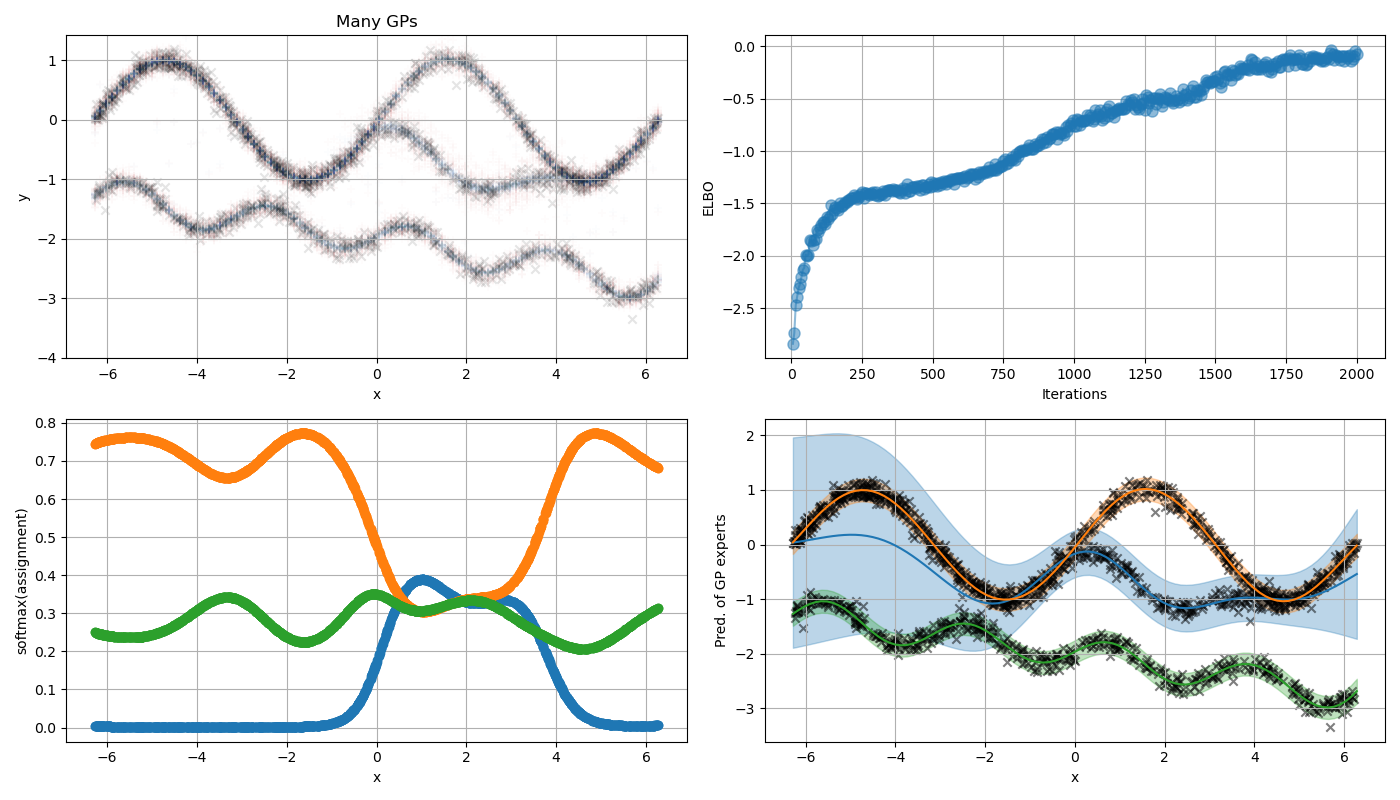
\includegraphics[width=\linewidth]{demo_tf2.png}
    \caption{Multimodal SMGP results on stochastic toy data}
    \label{fig:MultimodalSMGP}
\end{figure}

\section{XGBoost}

\begin{table}[H] \label{tab:XGResults}
	\centering
	\caption{Results of XGBoost model}
	\begin{tabular}{| c | c | c |} 
		\hline
		Model Features & \% Accuracy & Log Loss \\ [0.5ex] 
		\hline\hline
		StumpsX \& StumpsY & 75.0 & 0.5796 \\
		\hline
		StumpsX \& StumpsY \& PitchX \& PitchY & 71.43 & 0.5811 \\ [1ex]
		\hline
	\end{tabular}
\end{table}

TODO: Talk about accuracy.

\begin{figure}[H]
    \centering
    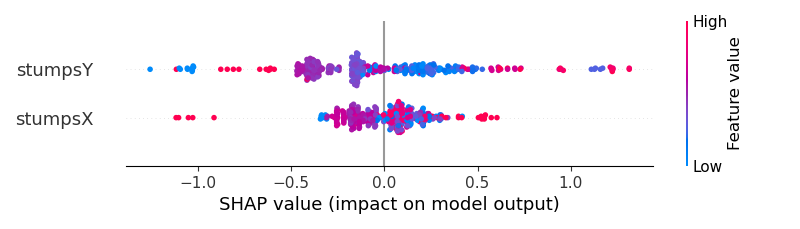
\includegraphics[width=\linewidth]{shap_stumps.png}
    \caption{SHAP values for XGBoost model with stumpsX and stumpsY as features}
    \label{fig:ShapStumps}
\end{figure}

\begin{figure}[H]
    \centering
    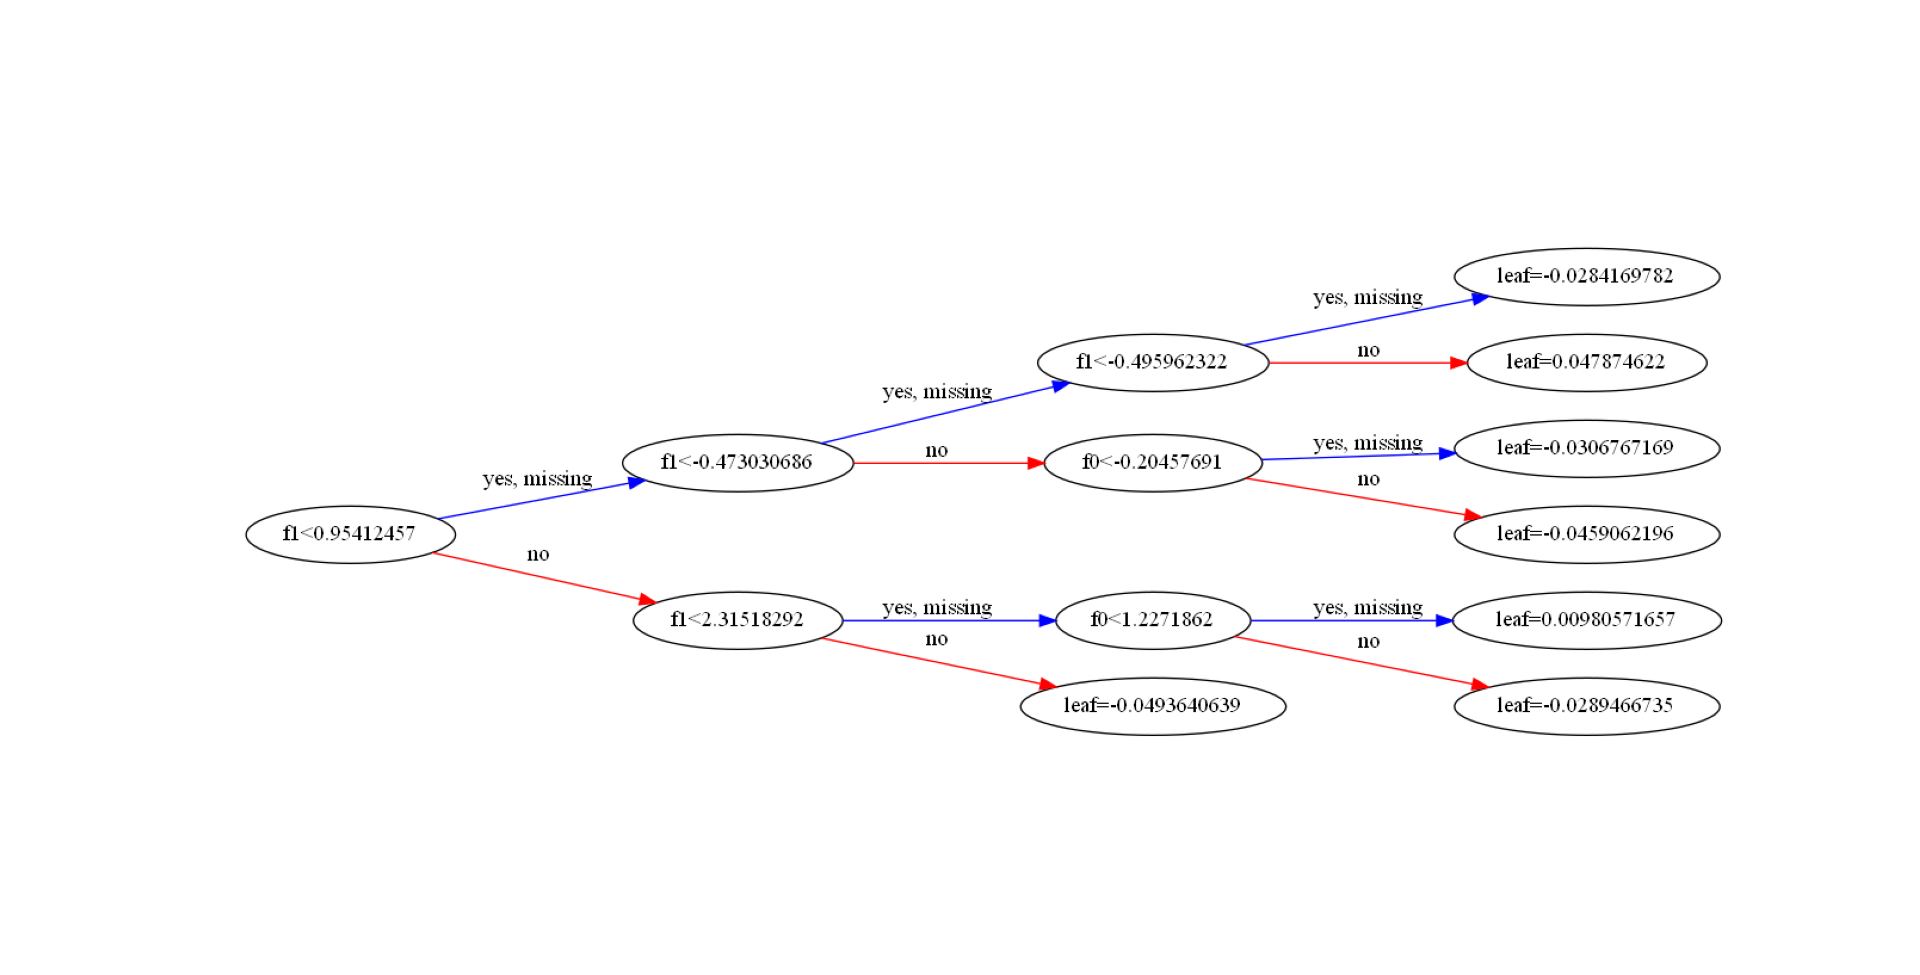
\includegraphics[width=\linewidth]{tree_stumps.png}
    \caption{Decision tree for XGBoost model with stumpsX and stumpsY as features}
    \label{fig:TreeStumps}
\end{figure}

XGBoost models can be difficult to interpret. 
The SHAP package offers a solution to interpreting XGBoost models, using principles of game theory to determine the effect of each feature on the odds of each outcome.
Essentially, SHAP considers how much the probabilities change when adding or removing features from the model.
Figure \ref{fig:ShapStumps} visualises the SHAP values for each feature, with a "high" shap value indicating a higher chance of scoring a six.
TODO: Flesh this out

\begin{figure}[H]
    \centering
    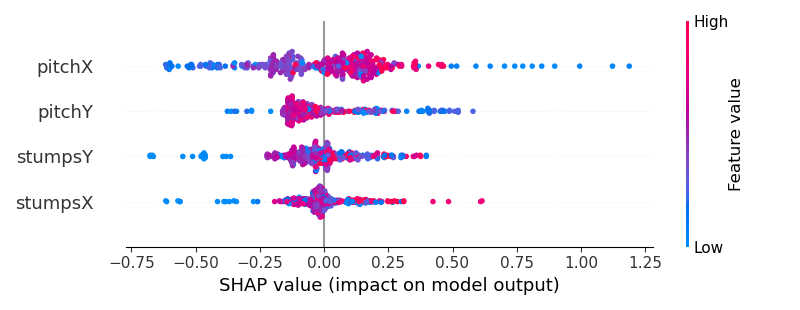
\includegraphics[width=\linewidth]{shap_stumps_pitch.png}
    \caption{SHAP values for XGBoost model with stumpsX, stumpsY, pitchX and pitchY as features}
    \label{fig:ShapStumpsPitch}
\end{figure}

\begin{figure}[H]
    \centering
    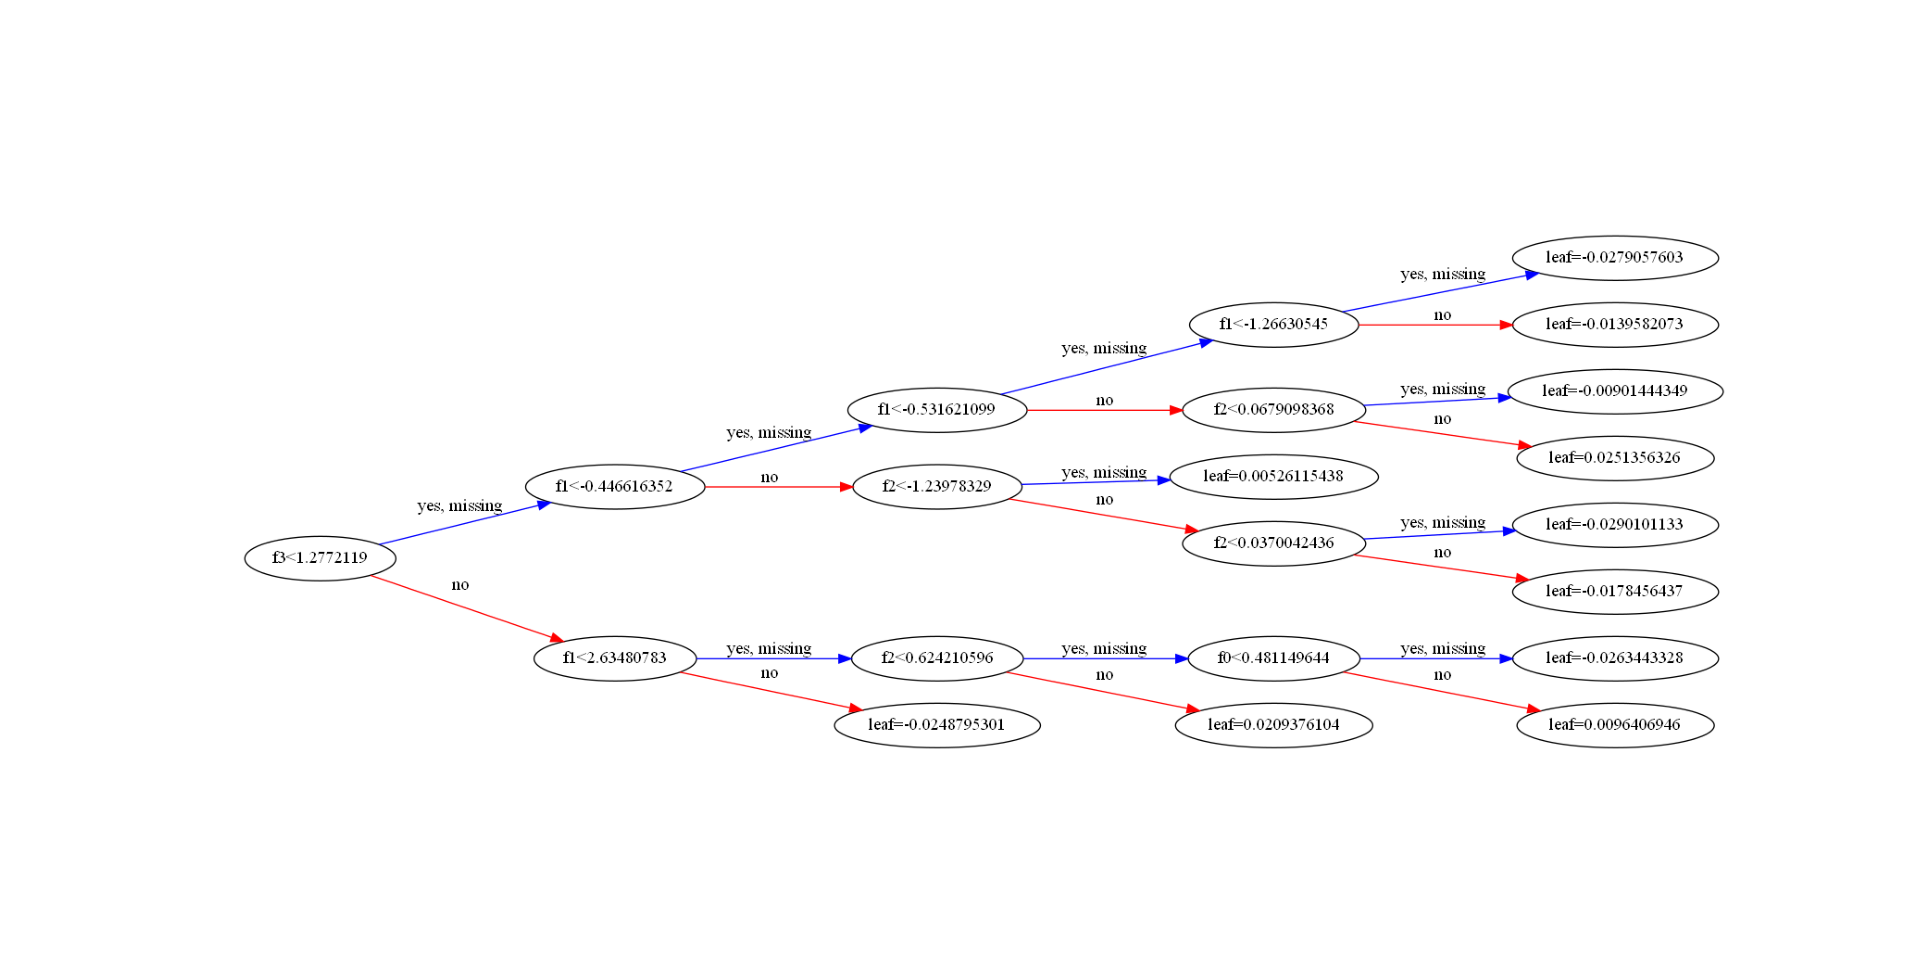
\includegraphics[width=\linewidth]{tree_stumps_pitch.png}
    \caption{Decision tree for XGBoost model with stumpsX, stumpsY, pitchX and pitchY as features}
    \label{fig:TreeStumpsPitch}
\end{figure}

%%%%%%%%%%%%%%%%%%%%%%%%%%%%%%%%%%%%%%%%%%%%%%%%%%%%%%%%%%%%%%%%%%%%%%%%%%%%%%%%
%%%%%%%%%%%%%%%%%%%%%%%%%%%%%%%%%%%%%%%%%%%%%%%%%%%%%%%%%%%%%%%%%%%%%%%%%%%%%%%%
\chapter{Discussion}

TODO: Discuss results and findings. Mention things discussed with Adam on slack etc.

%%%%%%%%%%%%%%%%%%%%%%%%%%%%%%%%%%%%%%%%%%%%%%%%%%%%%%%%%%%%%%%%%%%%%%%%%%%%%%%%
%%%%%%%%%%%%%%%%%%%%%%%%%%%%%%%%%%%%%%%%%%%%%%%%%%%%%%%%%%%%%%%%%%%%%%%%%%%%%%%%
\chapter{Conclusion}

TODO: Conclude on results and findings. Explain future work (e.g. taking into account that we know the assignments). Furthermore more inputs and use of categorical inputs etc.

\section{Future Work}

%%%%%%%%%%%%%%%%%%%%%%%%%%%%%%%%%%%%%%%%%%%%%%%%%%%%%%%%%%%%%%%%%%%%%%%%%%%%%%%%
%%%%%%%%%%%%%%%%%%%%%%%%%%%%%%%%%%%%%%%%%%%%%%%%%%%%%%%%%%%%%%%%%%%%%%%%%%%%%%%%

%Code can be output inline using \verb@\lstinline|some code|@.  For example, this code is inline: \lstinline|public static int example = 0;| (we have used the character \verb@|@ as a delimiter, but any non-reserved character not in the code text can be used.)
%
%Code snippets can be output using the \verb|\begin{lstlisting} ... \end{lstlisting}|
%environment with the code given in the environment. For example, consider listing \ref{Example-Code}, below.
%
%\begin{lstlisting}[breaklines,breakatwhitespace,caption={Example code},label=Example-Code]
%public static void main() {
%
%  System.out.println("Hello World");
%
%}
%\end{lstlisting}
%
%Code listings are produced using the package `listings'.  This has many useful options, so have a look at the package documentation for further ideas.
%
%\section[Short Section Title]{Another Section With a Long Title and Whose Title Is Abbreviated in the Table of Contents}
%
%%-------------------------------------------------------------------------------
%\begin{table}[htb]
%\caption{An example table}
%\bigskip
%\begin{center}
%\label{Example-Table}
%\begin{tabular}{|l|l|}
%\hline
%Items & Values \\
%\hline
%\hline
%Item 1 & Value 1 \\
%Item 2 & Value 2 \\
%\hline
%\end{tabular}
%\end{center}
%\end{table}
%
%Another section, just for good measure. You can reference a table, figure or equation using \verb|\ref|, just like this reference to Table \ref{Example-Table}.
%
%%%%%%%%%%%%%%%%%%%%%%%%%%%%%%%%%%%%%%%%%%%%%%%%%%%%%%%%%%%%%%%%%%%%%%%%%%%%%%%%%
%\section{Example Lists}
%
%%-------------------------------------------------------------------------------
%\subsection{Enumerated}
%
%\begin{enumerate}
%\item Example enumerated list:
%  \begin{itemize}
%  \item a nested enumerated list item;
%  \item and another one.
%  \end{itemize}
%\item Second item in the list.
%\end{enumerate}
%
%%-------------------------------------------------------------------------------
%\subsection{Itemised}
%
%\begin{itemize}
%\item Example itemised list.
%  \begin{itemize}
%  \item A nested itemised list item.
%  \end{itemize}
%\item Second item in the list.
%\end{itemize}
%
%%-------------------------------------------------------------------------------
%\subsection{Description}
%
%\begin{description}
%\item[Item 1]First item in the list.
%\item[Item 2]Second item in the list.
%\end{description}

% IGNORE WORDS AFTER HERE
%TC:ignore 

%%%%%%%%%%%%%%%%%%%%%%%%%%%%%%%%%%%%%%%%%%%%%%%%%%%%%%%%%%%%%%%%%%%%%%%%%%%%%%%%
%%%%%%%%%%%%%%%%%%%%%%%%%%%%%%%%%%%%%%%%%%%%%%%%%%%%%%%%%%%%%%%%%%%%%%%%%%%%%%%%
\bibliography{BibFile}

%%%%%%%%%%%%%%%%%%%%%%%%%%%%%%%%%%%%%%%%%%%%%%%%%%%%%%%%%%%%%%%%%%%%%%%%%%%%%%%%
%%%%%%%%%%%%%%%%%%%%%%%%%%%%%%%%%%%%%%%%%%%%%%%%%%%%%%%%%%%%%%%%%%%%%%%%%%%%%%%%
\appendix

%%
%% Use the appendix for major chunks of detailed work, such as these. Tailor
%% these to your own requirements
%%

\chapter{Cricket Background} \label{chap:CrickBackground}

Whilst knowledge of cricket is useful to understand this project, I do not deem it necessary to appreciate the project and its applications.
Any key ideas around cricket, T20 and IPL beyond the laws of the game are introduced in the main report.
Despite this, I present a brief introduction to the game and its laws for those unfamiliar with the sport.
Certain aspects of cricket have been introduced in limited detail, such as fielding and umpiring as they are unnecessary to understand in detail for this project.

\section{A Brief Overview of Cricket}

Cricket is a bat and ball game played between two teams of eleven players. 
It is played on a field, the centre of which is a pitch with wickets at each end comprising two bails balanced on three stumps. 
At the edge of the field is a boundary rope, see section \ref{sec:Boundaries}. 
The batting side scores runs by hitting the ball bowled at one of the wickets and then running between the wickets, or scoring a boundary.
The fielding side tries to prevent this, by getting the ball to either wicket and dismissing the batters so they are "out", see section \ref{sec:Dismissals}.
Which side bats/fields first is determined before the match starts through a coin toss between both team captains.
When ten batters have been dismissed, the innings ends and the teams swap sides (the fielding side bat, and the batting side field).
The game is referreed by two umpires.
In the case of international or professional cricket, there is typically an additional 3rd umpire off the field for video or technology assisted reviews.

\section{Additional T20 Cricket Details} \label{sec:AdditionalT20Cricket}

The following section includes any additional details on T20 cricket not included in section \ref{sec:T20Cricket}.

\subsection{Super Overs}

On the rare case a T20 game finishes with both sides scoring the same number of runs, a tie breaker "super over" is played.
In a super over, each team nominates three batsmen and one bowler to play a one-over-per-side "mini-match".
If the Super Over also ends up in a tie, it is repeated until the tie is broken.
An \emph{over} is a set of 6 fair deliveries (so not wides and no balls, see section \ref{sec:Overs}) for the batting team to score.

\section{Laws and Gameplay}

\subsection{Playing Field}

\begin{figure}[H]
    \centering
    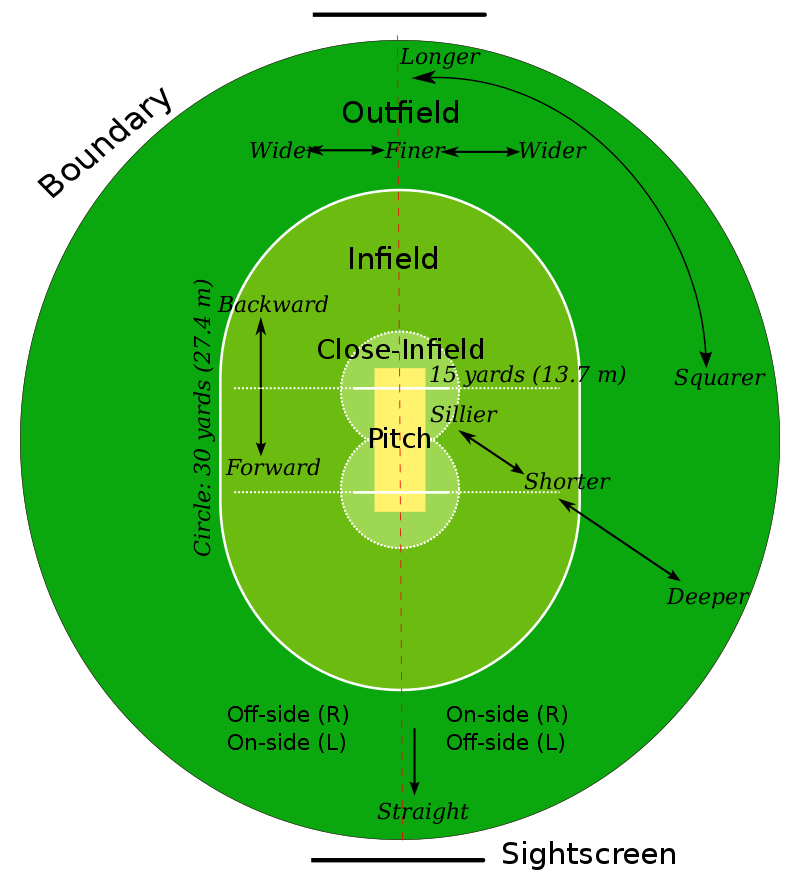
\includegraphics[width=0.8\linewidth]{Cricket_Field.png}
    \caption{A typical cricket field \citep{cricketWiki}}
    \label{fig:CricketField}
\end{figure}

A cricket field as mentioned, comprises a central pitch with wickets at both ends of the pitch. 
A wicket is three stumps, with two bails balanced on top. 
See figure \ref{fig:CricketField} for a visual representation.
The boundary surrounds the edge of the field and typically the field is oval in shape.

\begin{figure}[H]
    \centering
    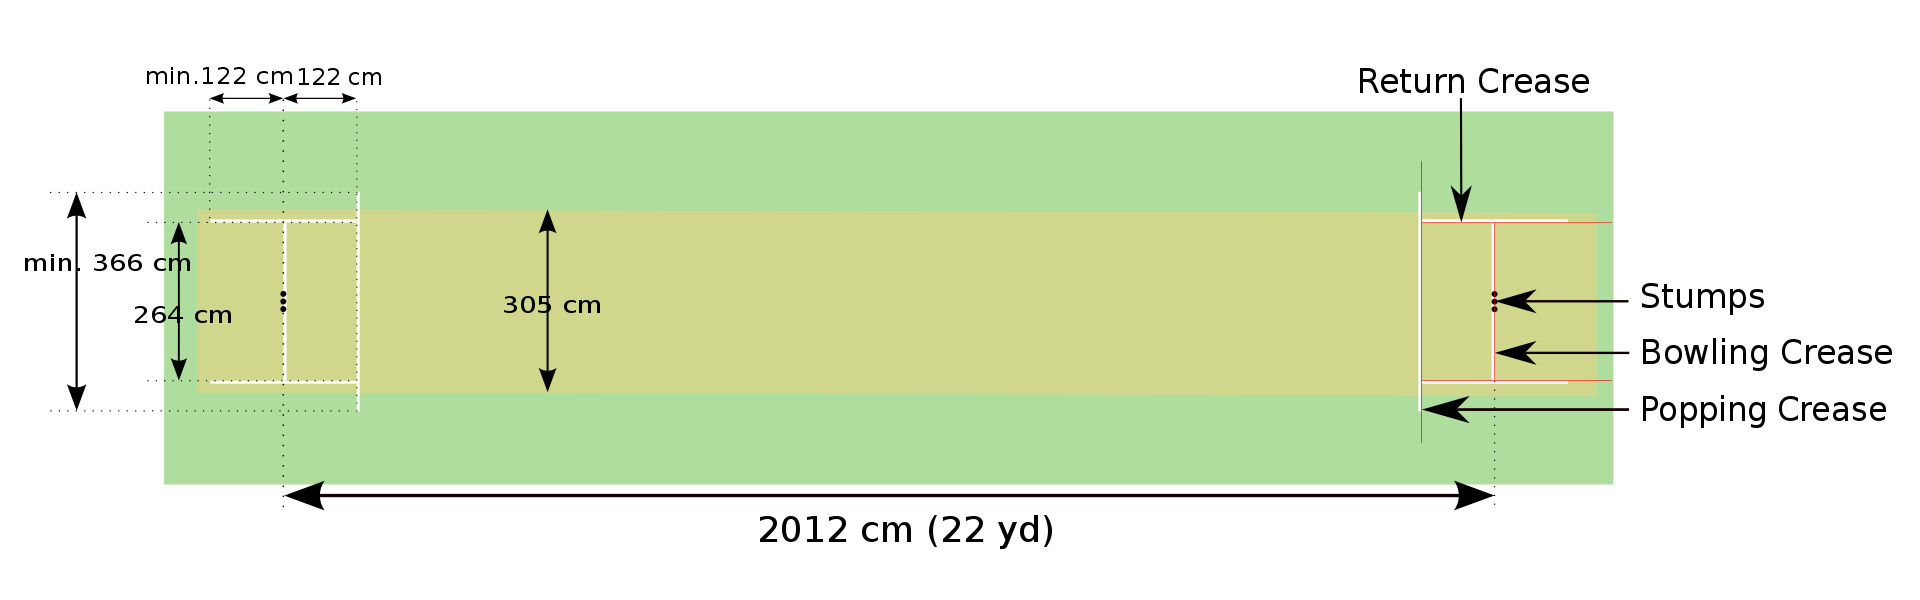
\includegraphics[width=0.8\linewidth]{Cricket_Pitch.png}
    \caption{A typical cricket pitch \citep{cricketWiki}}
    \label{fig:CricketPitch}
\end{figure}

Figure \ref{fig:CricketPitch} shows a cricket pitch including the location of the wickets and the creases.
As illustrated, the pitch is marked at each end with four white painted lines: a bowling crease, a popping crease and two return creases.

\subsection{Runs} \label{sec:Runs}

Runs are scored through either boundaries, or batsmen running between the creases.
For the latter, the batter on strike attempts to score runs by hitting the ball whilst simultaneously not getting out. 
To score runs, after the batsmen strikes the ball there needs to be enough time for the batsmen at both ends to run to the other end of the wicket.
If the fielding team get the ball to the wickets before the batsmen they could be \emph{run out}, see section \ref{sec:Dismissals}.
To register a run, both runners must touch the ground behind the popping crease with either their bats or their bodies (the batters carry their bats as they run). 
Each completed run increments the score of both the team and the striker.
Infinitely many runs can be scored off one delivery this way, with the batsmen running back and forth between the wickets.
Typically the maxmimum runs scored this way would be three, but it is possible to score more if there are misfields.

TODO:  Explain definition of dot ball and single.

\subsubsection{Boundaries} \label{sec:Boundaries}

A boundary is scored when the ball is hit by the batsmen all the way to the boundary rope.
Four runs are scored if the ball touches the ground at all prior to crossing the rope. 
If the ball is hit all the way over the boundary rope before touching the ground this is six runs. 
In T20 cricket the batsmen will typically aim to score boundaries, as they have the maximum return of runs.

\subsubsection{Extras}

Additional runs can be gained by the batting team as extras due to errors made by the fielding team. 
This is achieved in four ways: no-balls, wides, byes, and leg byes. 
A no ball occurs if the bowler bowls an illegal delivery, most commonly by overstepping the crease, but can also be called by an umpire for dangerous bowling.
In T20 cricket and IPL, no balls award the batting team a \emph{free hit}, a delivery in which they can only be dismissed via run out, hit the ball twice and obstructing the field (see section \ref{sec:Dismissals}).
A wide has occured if the bowler bowls so that the ball is out of reach of the batter.
Both a wide and a no ball have to be re-bowled and award the batting team one run.
Byes are any runs the batters achieve without hitting the ball, typically when the ball has been missed by the wicket keeper.
Leg byes are any runs the batters achieve when the ball hits their body, but not their bat.

\subsection{Overs} \label{sec:Overs}

An over is 6 fair deliveries (not including wides and no balls etc.).
A bowler can not bowl 2 overs in a row and at the end of an over the bowling end on the pitch changes. 
Despite this, typically bowlers will bowl in \emph{spells}, where they will bowl alternate overs from the same end.
In T20 cricket a bowler can bowl a maximum of 4 overs, meaning a minimum of 5 bowlers must be used. 
Typically a bowler might bowl two 2 over spells, however sometimes spinners in the middle of an innings might bowl all of their 4 overs in one spell.
Unlike bowlers, the batsmen do not change ends at the end of each over. 

\subsection{Dismissals} \label{sec:Dismissals}

There are nine ways a batter can be dismissed in cricket. 
The most common include being bowled, caught, leg before wicket (lbw), run out and stumped. 
Less common dismissals include hit wicket, hit the ball twice, obstructing the field, and timed out. 
For the purpose of this chapter I will only explain the most common dismissals. 

\begin{figure}[H]
    \centering
    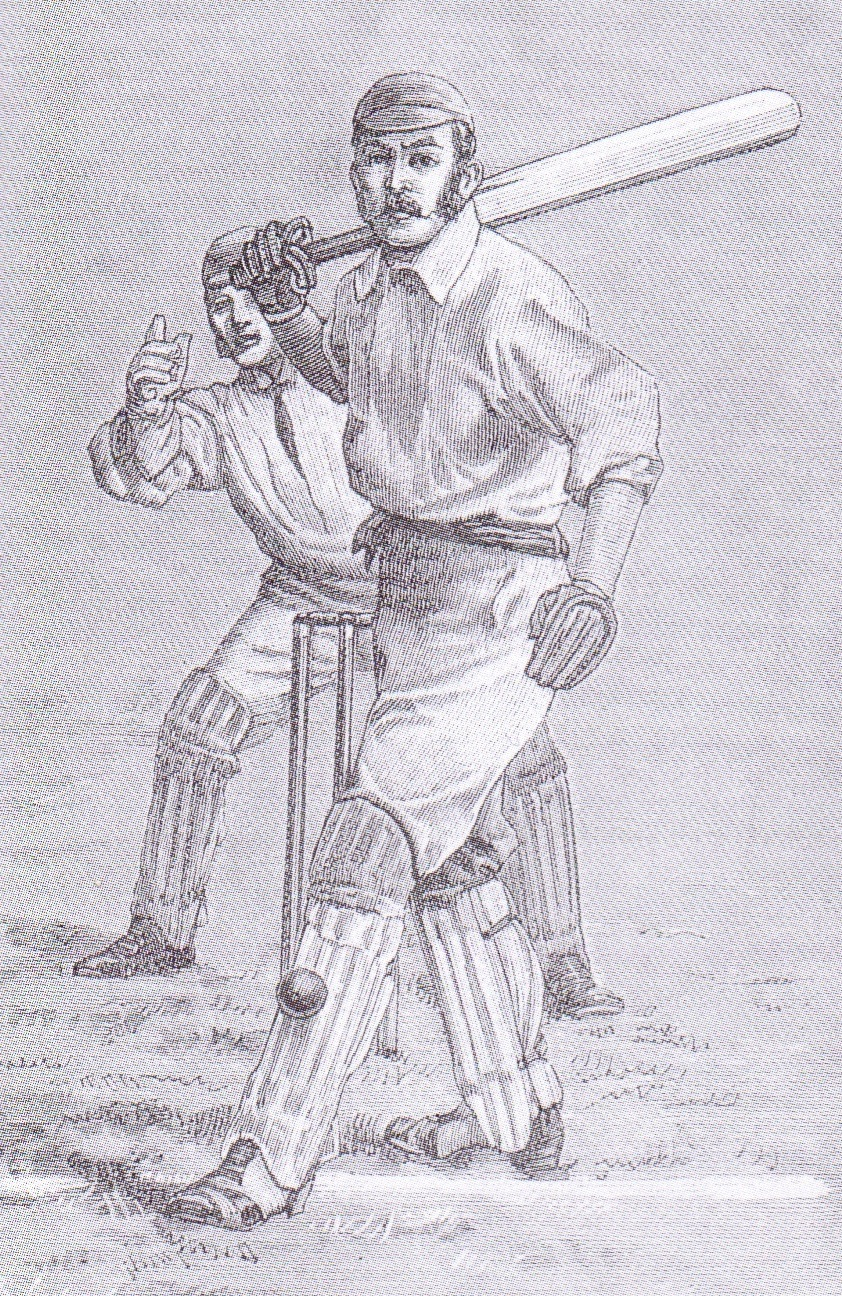
\includegraphics[width=0.8\linewidth]{Leg_before_wicket.jpg}
    \caption{A clear example of leg before wicket (lbw) \citep{lbwWiki}}
    \label{fig:lbw}
\end{figure}

\subsubsection{Bowled}

Being bowled is when the batter misses the delivery and the ball hits the stumps and takes the bails off the wickets.
If the bails do not come off the wickets, the batter is not out, though this is very rare.

\subsubsection{Caught}

Being caught is when the batter strikes the ball in the air and a fielder catches this before the ball touches the ground.
If the ball touches the ground at any stage (even in the fielders hands) it is not out.

\subsubsection{Leg Before Wicket (lbw)}

Leg before wicket is a more complicated dimissal type.
Following an appeal by the fielding side, the umpire may rule a batter out lbw if the ball would have struck the wicket but was instead intercepted by any part of the batter's body (except the hand holding the bat). 
The umpire's decision will depend on a number of criteria, including where the ball pitched, whether the ball hit in line with the wickets, the ball's expected future trajectory after hitting the batsman, and whether the batter was attempting to hit the ball.
Without explaining the finer details of lbw, a clear example of lbw is illustrated in figure \ref{fig:lbw}. 
Further information on lbw can be found on \citet{lbwWiki}.

\subsubsection{Run Out}

A run out usually occurs when the batters are attempting to run between the wickets.
The fielding team must successfully get the ball to one wicket and take the bails off with the ball (or their hands with the ball in them) before a batter has crossed the crease line near the wicket. 
The incomplete run the batters were attempting does not count.

\subsubsection{Stumped}

Lastly, being stumped involves the wicket-keeper catching the ball after the delivery and taking the bails of the stumps with the ball (or their hands with the ball in them) while the batsman is out of his ground (the batsman leaves his ground when he has moved down the pitch beyond the popping crease, usually in an attempt to hit the ball).
A batter can only be stumped off a fair delivery (not a no ball or a wide).
It is a special case of being run out and can only be performed by the fielding wicket keeper.

\subsection{Basic Gameplay Example}

\begin{figure}[H]
    \centering
    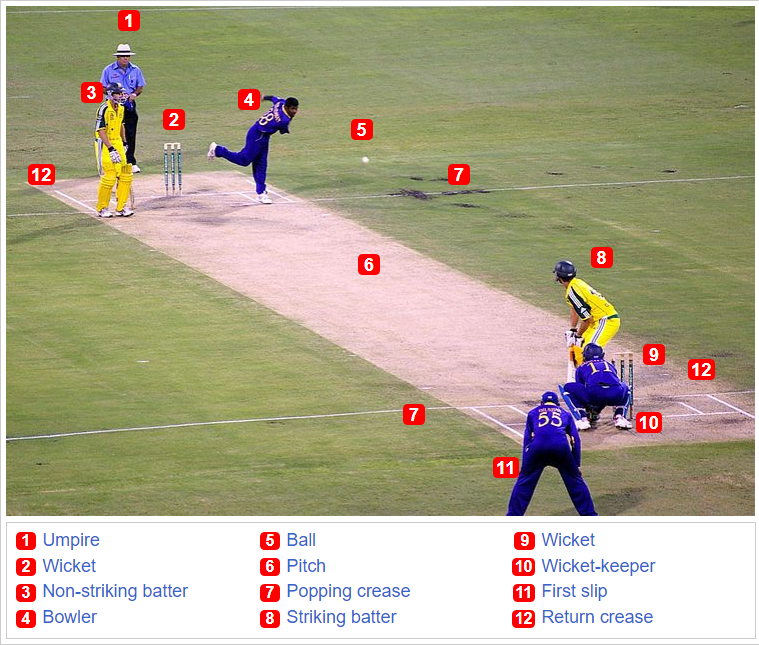
\includegraphics[width=0.8\linewidth]{Cricket_Delivery.png}
    \caption{An example of a ball being bowled and the components in play \citep{cricketWiki}}
    \label{fig:Delivery}
\end{figure}

Figure \ref{fig:Delivery} shows a cricket delivery in play. 
The two batters (3 and 8; wearing yellow) have taken position at each end of the pitch (6). 
Three members of the fielding team (4, 10 and 11; wearing dark blue) are in shot. 
The bowler (4) is bowling the ball (5) from his end of the pitch to the batter (8) at the other end who is called the "striker". 
The other batter (3) at the bowling end is called the "non-striker". 
The wicket-keeper (10) is positioned behind the striker's wicket (9).

The bowler (4) intends to dimiss the batsmen, or to prevent the striker (8) from scoring runs. 
By using his bat, the striker (8) intends to defend his wicket and hit the ball away from the pitch in order to score runs.

\subsection{Player Roles}

Typically players are selected to perform a specialised role.

\subsubsection{Bowlers}

As mentioned a minimum of five bowlers are required to bowl in a T20 match.  
Therefore, team selectors will typically choose 5-6 bowlers for the team for a given match.
A bowler is someone specialised for bowling in one of two main ways: Seam (pace) bowling, or spin bowling.
Seam bowlers typically use techniques such as \emph{swing} or \emph{seam} paired with a higher bowling speed (generally anywhere from 70 - 95 mph) to try and get wickets or reduce the runs scored.
However, in T20 cricket, seam bowlers will typically use a wider variety of delivery types, including slower balls, yorkers, bouncers, slower ball bouncers, wide yorkers, cross seam and more, to make prediciting their bowling more difficult and reduce the runs scored. 
Spin bowlers come in two main varieties: off spinners or leg spinners, and this essentially means what way they spin the ball. 
To spin the ball means to get the ball the ball to move dramatically in one direction after its bounce, by spinning it on release from the bowlers hand.
Due to trying to spin the ball, spinners will typically bowl at a slower speed than pace bowlers (generally 45 - 65 mph).
Like pace bowlers, a spin bowler in T20 cricket will use a variety of delivery types to try and reduce the runs scored from the opposing team.

\subsubsection{Batters}

The other main role is that of a batter.
A batters job is to score runs for their team.
In T20 cricket batters are generally specialised to score boundaries due to the short format, rather than be particularly good at protecting their wicket and staying in bat for many hours.

\subsubsection{Wicket Keepers}

The wicket keeper is a specialist fielder who stands behind the stumps to field the ball after it has been bowled.
In the modern game, they are expected to also be reasonably good batsmen regardless of their wicket keeping skill.

\subsubsection{All Rounders}

All rounders are a special player who are good at both batting and bowling.
All rounders are valued players, as they can provide the role of both a batter and bowler whilst only taking up one space on the teamsheet.

\subsubsection{Captain}

The last specialist role I will cover is that of the captain. 
The captain performs their captain duties as a batter, bowler, wicket keeper, or all rounder, while taking on the additional captains duties.
The captain decides who will bowl each over and where each fielder will be positioned. 
While decisions are often collaborative, the captain has the final say.
Captains in cricket typically shoulder more responsibility on the outcome of a cricket match than captains in other sports, given their level of responsibilty.

%%%%%%%%%%%%%%%%%%%%%%%%%%%%%%%%%%%%%%%%%%%%%%%%%%%%%%%%%%%%%%%%%%%%%%%%%%%%%%%%
%%%%%%%%%%%%%%%%%%%%%%%%%%%%%%%%%%%%%%%%%%%%%%%%%%%%%%%%%%%%%%%%%%%%%%%%%%%%%%%%
\chapter{Mathematical Background}

\section{Cholesky Factorisation} \label{sec:CholFac}

TODO: Cholesky Factorisation

\section{Kullback–Leibler Divergence} \label{sec:KLDiv}

TODO: KL Divergence

%%%%%%%%%%%%%%%%%%%%%%%%%%%%%%%%%%%%%%%%%%%%%%%%%%%%%%%%%%%%%%%%%%%%%%%%%%%%%%%%
%%%%%%%%%%%%%%%%%%%%%%%%%%%%%%%%%%%%%%%%%%%%%%%%%%%%%%%%%%%%%%%%%%%%%%%%%%%%%%%%
\chapter{Code}

%STOP IGNORING WORDS
%TC:endignore 

\end{document}
